% Options for packages loaded elsewhere
\PassOptionsToPackage{unicode}{hyperref}
\PassOptionsToPackage{hyphens}{url}
\PassOptionsToPackage{dvipsnames,svgnames,x11names}{xcolor}
%
\documentclass[
  a4paper,
]{scrreport}

\usepackage{amsmath,amssymb}
\usepackage{iftex}
\ifPDFTeX
  \usepackage[T1]{fontenc}
  \usepackage[utf8]{inputenc}
  \usepackage{textcomp} % provide euro and other symbols
\else % if luatex or xetex
  \usepackage{unicode-math}
  \defaultfontfeatures{Scale=MatchLowercase}
  \defaultfontfeatures[\rmfamily]{Ligatures=TeX,Scale=1}
\fi
\usepackage{lmodern}
\ifPDFTeX\else  
    % xetex/luatex font selection
\fi
% Use upquote if available, for straight quotes in verbatim environments
\IfFileExists{upquote.sty}{\usepackage{upquote}}{}
\IfFileExists{microtype.sty}{% use microtype if available
  \usepackage[]{microtype}
  \UseMicrotypeSet[protrusion]{basicmath} % disable protrusion for tt fonts
}{}
\makeatletter
\@ifundefined{KOMAClassName}{% if non-KOMA class
  \IfFileExists{parskip.sty}{%
    \usepackage{parskip}
  }{% else
    \setlength{\parindent}{0pt}
    \setlength{\parskip}{6pt plus 2pt minus 1pt}}
}{% if KOMA class
  \KOMAoptions{parskip=half}}
\makeatother
\usepackage{xcolor}
\setlength{\emergencystretch}{3em} % prevent overfull lines
\setcounter{secnumdepth}{5}
% Make \paragraph and \subparagraph free-standing
\ifx\paragraph\undefined\else
  \let\oldparagraph\paragraph
  \renewcommand{\paragraph}[1]{\oldparagraph{#1}\mbox{}}
\fi
\ifx\subparagraph\undefined\else
  \let\oldsubparagraph\subparagraph
  \renewcommand{\subparagraph}[1]{\oldsubparagraph{#1}\mbox{}}
\fi


\providecommand{\tightlist}{%
  \setlength{\itemsep}{0pt}\setlength{\parskip}{0pt}}\usepackage{longtable,booktabs,array}
\usepackage{calc} % for calculating minipage widths
% Correct order of tables after \paragraph or \subparagraph
\usepackage{etoolbox}
\makeatletter
\patchcmd\longtable{\par}{\if@noskipsec\mbox{}\fi\par}{}{}
\makeatother
% Allow footnotes in longtable head/foot
\IfFileExists{footnotehyper.sty}{\usepackage{footnotehyper}}{\usepackage{footnote}}
\makesavenoteenv{longtable}
\usepackage{graphicx}
\makeatletter
\def\maxwidth{\ifdim\Gin@nat@width>\linewidth\linewidth\else\Gin@nat@width\fi}
\def\maxheight{\ifdim\Gin@nat@height>\textheight\textheight\else\Gin@nat@height\fi}
\makeatother
% Scale images if necessary, so that they will not overflow the page
% margins by default, and it is still possible to overwrite the defaults
% using explicit options in \includegraphics[width, height, ...]{}
\setkeys{Gin}{width=\maxwidth,height=\maxheight,keepaspectratio}
% Set default figure placement to htbp
\makeatletter
\def\fps@figure{htbp}
\makeatother

\usepackage{pgfplots}
\usetikzlibrary{arrows.meta,arrows}
\usetikzlibrary{shapes.geometric}
\usetikzlibrary{angles,quotes}
\pgfplotsset{grid style={dashed,mygray}}
% Colors
\definecolor{myblue}{rgb}{0.067,0.529,0.871}
\definecolor{mypurple}{rgb}{0.859,0.071,0.525}
\definecolor{myred}{rgb}{1.0, 0.13, 0.32}
\definecolor{mygreen}{rgb}{0.01, 0.75, 0.24}
\definecolor{myblack}{gray}{0.1}
\definecolor{mygray}{gray}{0.8}
\newcommand{\NN}{\mathbb{N}}
\newcommand{\ZZ}{\mathbb{Z}}
\newcommand{\QQ}{\mathbb{Q}}
\newcommand{\RR}{\mathbb{R}}
\newcommand{\CC}{\mathbb{C}}
\DeclareMathOperator{\Int}{Int}
\DeclareMathOperator{\Ext}{Ext}
\DeclareMathOperator{\Fr}{Fr}
\DeclareMathOperator{\Adh}{Adh}
\DeclareMathOperator{\Ac}{Ac}
\DeclareMathOperator{\sen}{sen}
\makeatletter
\@ifpackageloaded{tcolorbox}{}{\usepackage[skins,breakable]{tcolorbox}}
\@ifpackageloaded{fontawesome5}{}{\usepackage{fontawesome5}}
\definecolor{quarto-callout-color}{HTML}{909090}
\definecolor{quarto-callout-note-color}{HTML}{0758E5}
\definecolor{quarto-callout-important-color}{HTML}{CC1914}
\definecolor{quarto-callout-warning-color}{HTML}{EB9113}
\definecolor{quarto-callout-tip-color}{HTML}{00A047}
\definecolor{quarto-callout-caution-color}{HTML}{FC5300}
\definecolor{quarto-callout-color-frame}{HTML}{acacac}
\definecolor{quarto-callout-note-color-frame}{HTML}{4582ec}
\definecolor{quarto-callout-important-color-frame}{HTML}{d9534f}
\definecolor{quarto-callout-warning-color-frame}{HTML}{f0ad4e}
\definecolor{quarto-callout-tip-color-frame}{HTML}{02b875}
\definecolor{quarto-callout-caution-color-frame}{HTML}{fd7e14}
\makeatother
\makeatletter
\@ifpackageloaded{tikz}{}{\usepackage{tikz}}
\makeatother
\makeatletter
\@ifpackageloaded{bookmark}{}{\usepackage{bookmark}}
\makeatother
\makeatletter
\@ifpackageloaded{caption}{}{\usepackage{caption}}
\AtBeginDocument{%
\ifdefined\contentsname
  \renewcommand*\contentsname{Tabla de contenidos}
\else
  \newcommand\contentsname{Tabla de contenidos}
\fi
\ifdefined\listfigurename
  \renewcommand*\listfigurename{Listado de Figuras}
\else
  \newcommand\listfigurename{Listado de Figuras}
\fi
\ifdefined\listtablename
  \renewcommand*\listtablename{Listado de Tablas}
\else
  \newcommand\listtablename{Listado de Tablas}
\fi
\ifdefined\figurename
  \renewcommand*\figurename{Figura}
\else
  \newcommand\figurename{Figura}
\fi
\ifdefined\tablename
  \renewcommand*\tablename{Tabla}
\else
  \newcommand\tablename{Tabla}
\fi
}
\@ifpackageloaded{float}{}{\usepackage{float}}
\floatstyle{ruled}
\@ifundefined{c@chapter}{\newfloat{codelisting}{h}{lop}}{\newfloat{codelisting}{h}{lop}[chapter]}
\floatname{codelisting}{Listado}
\newcommand*\listoflistings{\listof{codelisting}{Listado de Listados}}
\usepackage{amsthm}
\theoremstyle{definition}
\newtheorem{exercise}{Ejercicio}[chapter]
\theoremstyle{remark}
\AtBeginDocument{\renewcommand*{\proofname}{Prueba}}
\newtheorem*{remark}{Observación}
\newtheorem*{solution}{Solución}
\makeatother
\makeatletter
\@ifpackageloaded{caption}{}{\usepackage{caption}}
\@ifpackageloaded{subcaption}{}{\usepackage{subcaption}}
\makeatother
\makeatletter
\@ifpackageloaded{tcolorbox}{}{\usepackage[skins,breakable]{tcolorbox}}
\makeatother
\makeatletter
\@ifundefined{shadecolor}{\definecolor{shadecolor}{rgb}{.97, .97, .97}}
\makeatother
\makeatletter
\makeatother
\makeatletter
\makeatother
\ifLuaTeX
\usepackage[bidi=basic]{babel}
\else
\usepackage[bidi=default]{babel}
\fi
\babelprovide[main,import]{spanish}
% get rid of language-specific shorthands (see #6817):
\let\LanguageShortHands\languageshorthands
\def\languageshorthands#1{}
\ifLuaTeX
  \usepackage{selnolig}  % disable illegal ligatures
\fi
\IfFileExists{bookmark.sty}{\usepackage{bookmark}}{\usepackage{hyperref}}
\IfFileExists{xurl.sty}{\usepackage{xurl}}{} % add URL line breaks if available
\urlstyle{same} % disable monospaced font for URLs
\hypersetup{
  pdftitle={Exámenes de Análisis Matemático},
  pdfauthor={Alfredo Sánchez Alberca},
  pdflang={es},
  colorlinks=true,
  linkcolor={blue},
  filecolor={Maroon},
  citecolor={Blue},
  urlcolor={Blue},
  pdfcreator={LaTeX via pandoc}}

\title{Exámenes de Análisis Matemático}
\author{Alfredo Sánchez Alberca}
\date{2022-01-11}

\begin{document}
\begin{titlepage}

%\AddToShipoutPicture*{\put(0,0){\includegraphics[scale=0.8]{img/background2}}} % Imagen de fondo, requiere el paquete eso-pic.
\begin{center}
\vspace*{5cm}

\Huge
{\textbf{\textsf{Exámenes de Análisis Matemático}}}

\vspace{0.5cm}
\LARGE
{\textbf{\textsf{}}}

\vspace{1.5cm}


\includegraphics[width=0.4\textwidth]{img/logos/sticker.png}
\end{center}

\vfill

\begin{flushleft}
\begin{tabular}{ll}

\includegraphics[width=0.1\textwidth]{img/logos/aprendeconalf.png} & \parbox[b]{5cm}{\Large\textsf{Alfredo
Sánchez
Alberca}\\ \textsf{asalber@ceu.es} \\ \textsf{https://aprendeconalf.es}}
\end{tabular}
\end{flushleft}
\end{titlepage}\ifdefined\Shaded\renewenvironment{Shaded}{\begin{tcolorbox}[interior hidden, sharp corners, breakable, boxrule=0pt, enhanced, borderline west={3pt}{0pt}{shadecolor}, frame hidden]}{\end{tcolorbox}}\fi

\renewcommand*\contentsname{Tabla de contenidos}
{
\hypersetup{linkcolor=}
\setcounter{tocdepth}{2}
\tableofcontents
}
\bookmarksetup{startatroot}

\hypertarget{prefacio}{%
\chapter*{Prefacio}\label{prefacio}}
\addcontentsline{toc}{chapter}{Prefacio}

\markboth{Prefacio}{Prefacio}

Colección de exámenes de Análisis Matemático Real del grado en
Ingeniería Matemática.

\bookmarksetup{startatroot}

\hypertarget{examen-de-anuxe1lisis-i}{%
\chapter{\texorpdfstring{2022-11-14 Examen de Análisis
I}{2022-11-14  Examen de Análisis I}}\label{examen-de-anuxe1lisis-i}}

\begin{exercise}[]\protect\hypertarget{exr-1}{}\label{exr-1}

Calcular los puntos de acumulación del conjunto
\(A=[0,1]\cup \left\{\frac{n}{n-1}: n\in\mathbb{N}, n\geq 2\right\}\).
¿Es un conjunto cerrado? ¿Y abierto?

\end{exercise}

\begin{tcolorbox}[enhanced jigsaw, coltitle=black, colbacktitle=quarto-callout-tip-color!10!white, bottomtitle=1mm, opacitybacktitle=0.6, breakable, bottomrule=.15mm, colframe=quarto-callout-tip-color-frame, toprule=.15mm, titlerule=0mm, arc=.35mm, colback=white, title=\textcolor{quarto-callout-tip-color}{\faLightbulb}\hspace{0.5em}{Solución}, leftrule=.75mm, rightrule=.15mm, opacityback=0, left=2mm, toptitle=1mm]

Veamos primero que todos los puntos del intervalo \([0,1]\) son puntos
de acumulación. Sea \(x\in[0,1]\). Entonces para cualquier
\(\varepsilon>0\), por la densidad de los números reales, el entorno
reducido \((x-\varepsilon,x+\varepsilon)\setminus\{x\}\) contiene puntos
de \([0,1]\), y por tanto \(x\) es un punto de acumulación de \([0,1]\).

Veamos ahora que el conjunto
\(B=\left\{\frac{n}{n-1}: n\in\mathbb{N}, n\geq 2\right\} = \left\{1+\frac{1}{n-1}: n\in\mathbb{N}, n\geq 2\right\}\)
solo tiene \(1\) como punto de acumulación. En primer lugar, \(1\) es
punto de acumulación, ya que para cualquier \(\varepsilon>0\),
\((1-\varepsilon, 1+\varepsilon)\setminus \{1\}\) contiene puntos de
\(A\). Para verlo, basta aplicar la propiedad arquimediana, por la que
existe \(n\in\mathbb{N}\) tal que \(\frac{1}{n}<\varepsilon\), de manera
que \(1+\frac{1}{n}<1+\varepsilon\), y por tanto
\((1-\varepsilon, 1+\varepsilon)\setminus \{1\}\cap B\neq \emptyset\).

Si \(x<1\), tomando \(\varepsilon=|x-1|\) el entorno reducido
\((x-\varepsilon, x+\varepsilon)\setminus\{x\}\) no contiene puntos de
\(B\). Del mismo modo, si \(x>2\), tomando \(\varepsilon=|x-2|\) el
entorno reducido \((x-\varepsilon, x+\varepsilon)\setminus\{x\}\)
tampoco contiene puntos de \(B\). Finalmente, si \(1<x\leq 2\), por la
propiedad arquimediana, existe \(n\in\mathbb{N}\) tal que
\(\frac{1}{n}\leq x<\frac{1}{n-1}\). Tomando
\(\varepsilon=\min(\{|x-\frac{1}{n}|,|x-\frac{1}{n-1}|\})\) también se
tiene que el entorno reducido
\((x-\varepsilon, x+\varepsilon)\setminus\{x\}\) no contiene puntos de
\(B\). Por tanto, \(1\) es el único punto de acumulación de \(B\).

Así pues, \(\operatorname{Ac}(A)=[0,1]\), y como
\(\operatorname{Ac}(A)\subseteq A\), \(A\) es cerrado ya que contienen a
todos sus puntos de acumulación (ver
\href{https://aprendeconalf.es/analisis-manual/topologia-reales.html\#thm-conjunto-cerrado-puntos-acumulacion}{teorema}),
y por tanto, no puede ser abierto ya que los únicos conjuntos cerrados y
abiertos a la vez son \(\mathbb{R}\) y \(\emptyset\).

\end{tcolorbox}

\begin{exercise}[]\protect\hypertarget{exr-2}{}\label{exr-2}

Dada la sucesión \(\left(\frac{1}{2^n}\right)_{n=1}^\infty\),

\begin{enumerate}
\def\labelenumi{\alph{enumi}.}
\tightlist
\item
  Calcular, si existen, el supremo, ínfimo, máximo y mínimo del conjunto
  de sus términos.
\item
  Demostrar que la sucesión converge a \(0\).
\end{enumerate}

\end{exercise}

\begin{tcolorbox}[enhanced jigsaw, coltitle=black, colbacktitle=quarto-callout-tip-color!10!white, bottomtitle=1mm, opacitybacktitle=0.6, breakable, bottomrule=.15mm, colframe=quarto-callout-tip-color-frame, toprule=.15mm, titlerule=0mm, arc=.35mm, colback=white, title=\textcolor{quarto-callout-tip-color}{\faLightbulb}\hspace{0.5em}{Solución}, leftrule=.75mm, rightrule=.15mm, opacityback=0, left=2mm, toptitle=1mm]

\begin{enumerate}
\def\labelenumi{\alph{enumi}.}
\item
  La sucesión es monótona decreciente, ya que \(\forall n\in\mathbb{N}\)
  \(2^n<2^{n+1}\), y por tanto,
  \(x_n=\frac{1}{2^n}<\frac{1}{2^{n+1}}=x_{n+1}\). Así pues, el primer
  término de la sucesión \(x_1=1/2\) es su máximo, y por tanto el
  supremo.

  Veamos ahora que \(0\) es ínfimo por reducción al absurdo. En primer
  lugar, \(0\) es una cota inferior de la sucesión, pues todos sus
  términos son positivos. Supongamos ahora que existe otra cota inferior
  \(c\in\mathbb{R}\) tal que \(c>0\). Por la propiedad arquimediana,
  existe \(n\in\mathbb{N}\) tal que \(\frac{1}{n}< c\). Ahora bien, como
  \(n<2^n\) \(\forall n\in\mathbb{N}\), se tiene que
  \(\frac{1}{2^n}<\frac{1}{n}< c\), por lo que el termino \(n\) de la
  sucesión es menor que \(c\), lo que contradice que sea cota inferior.
  Así pues, \(0\) es el ínfimo. Sin embargo, la sucesión no tiene
  mínimo, pues \(x_n\neq 0\) \(\forall n\in\mathbb{N}\).
\item
  Como la sucesión es monótona decreciente y está acotada inferiormente,
  por el
  \href{https://aprendeconalf.es/analisis-manual/sucesiones.html\#thm-convergencia-monotona}{teorema
  de la convergencia de una sucesión monónota} la sucesión converge y
  \(\lim_{n\to\infty}x_n = \inf(\{x_n:n\in\mathbb{N}\})=0\).
\end{enumerate}

\end{tcolorbox}

\begin{exercise}[]\protect\hypertarget{exr-3}{}\label{exr-3}

La rentabilidad de un bono cada año, en porcentaje, viene dada por la
sucesión recurrente \(x_1=3\) y \(x_{n+1}=\sqrt{\frac{x_n}{2}+3}\).
¿Hacia dónde converge la rentabilidad del bono a medida que pasa el
tiempo?

\end{exercise}

\begin{tcolorbox}[enhanced jigsaw, coltitle=black, colbacktitle=quarto-callout-tip-color!10!white, bottomtitle=1mm, opacitybacktitle=0.6, breakable, bottomrule=.15mm, colframe=quarto-callout-tip-color-frame, toprule=.15mm, titlerule=0mm, arc=.35mm, colback=white, title=\textcolor{quarto-callout-tip-color}{\faLightbulb}\hspace{0.5em}{Solución}, leftrule=.75mm, rightrule=.15mm, opacityback=0, left=2mm, toptitle=1mm]

Veamos que primero que la sucesión es monótona decreciente.
\(x_1=3>x_n= \sqrt{\frac{3}{2}+3} = 2.12\). Supongamos ahora que
\(x_{n-1}>x_n\). Entonces

\begin{align*}
x_{n-1}>x_n &\Rightarrow \frac{x_{n-1}} {2}>\frac{x_n}{2} \Rightarrow \frac{x_{n-1}}{2}+3>\frac{x_n}{2}+3\\  & \Rightarrow \sqrt{\frac{x_{n-1}}{2}+3}>\sqrt{\frac{x_n}{2}+3} \Rightarrow x_n>x_{n+1}.
\end{align*} \[
\]

Por otro lado, es fácil ver que la sucesión está acotada inferiormente
por \(0\) pues todos los términos son positivos. Así pues, por el
\href{https://aprendeconalf.es/analisis-manual/sucesiones.html\#thm-convergencia-monotona}{teorema
de la convergencia de una sucesión monónota}, la sucesión converge a un
número \(x\in\mathbb{R}\). Para calcular el límite, aprovechando la
recurrencia de la sucesión se tiene

\[
x=\lim_{n\to\infty} x_n = \lim_{n\to\infty} x_{n+1} = \lim_{n\to\infty} \sqrt{\frac{x_n}{2}+3} = \sqrt{\lim_{n\to\infty}\frac{x_n}{2}+3} = \sqrt{\frac{x}{2}+3}
\]

Así pues, se cumple que \(x=\sqrt{\frac{x}{2}+3}\), y de ello se deduce

\[
x=\sqrt{\frac{x}{2}+3} \Rightarrow x^2=\frac{x}{2}+3 \Rightarrow x^2-3 = \frac{x}{2} \Rightarrow 2x^2-x-6 =0,\]

y resolviendo la ecuación se tiene \(x=-3/2\) y \(x=2\). Como todos los
términos de la sucesión son positivos, es imposible que converja a
\(-3/2\), y por tanto la rentabilidad del bono converge al \(2\)\%.

\end{tcolorbox}

\begin{exercise}[]\protect\hypertarget{exr-4}{}\label{exr-4}

Demostrar, usando la definición de límite, que
\(\lim_{x\to 1}\frac{3x+1}{2}=2\).

\end{exercise}

\begin{tcolorbox}[enhanced jigsaw, coltitle=black, colbacktitle=quarto-callout-tip-color!10!white, bottomtitle=1mm, opacitybacktitle=0.6, breakable, bottomrule=.15mm, colframe=quarto-callout-tip-color-frame, toprule=.15mm, titlerule=0mm, arc=.35mm, colback=white, title=\textcolor{quarto-callout-tip-color}{\faLightbulb}\hspace{0.5em}{Solución}, leftrule=.75mm, rightrule=.15mm, opacityback=0, left=2mm, toptitle=1mm]

Para cualquier \(\varepsilon>0\) existe
\(\delta=\frac{2}{3}\varepsilon\), tal que si
\(|x-1|<\delta=\frac{2}{3}\varepsilon\) se tiene

\[
\left|\frac{3x+1}{2}-2\right|= \left|\frac{3x+1-4}{2}\right| = \left|\frac{3x-3}{2}\right| = \left|\frac{3(x-1)}{2}\right| = \frac{3}{2}|x-1|< \frac{3}{2}\frac{2}{3}\varepsilon = \varepsilon.
\]

\end{tcolorbox}

\begin{exercise}[]\protect\hypertarget{exr-5}{}\label{exr-5}

Sabiendo que \(\lim_{x\to 0}(1+x)^{1/x}=e\), demostrar que las
siguientes funciones son infinitésimos equivalentes en \(x=0\):

\begin{enumerate}
\def\labelenumi{\alph{enumi}.}
\tightlist
\item
  \(\ln(1+x)\) y \(x\).
\item
  \(e^x-1\) y \(x\).
\end{enumerate}

\end{exercise}

\begin{tcolorbox}[enhanced jigsaw, coltitle=black, colbacktitle=quarto-callout-tip-color!10!white, bottomtitle=1mm, opacitybacktitle=0.6, breakable, bottomrule=.15mm, colframe=quarto-callout-tip-color-frame, toprule=.15mm, titlerule=0mm, arc=.35mm, colback=white, title=\textcolor{quarto-callout-tip-color}{\faLightbulb}\hspace{0.5em}{Solución}, leftrule=.75mm, rightrule=.15mm, opacityback=0, left=2mm, toptitle=1mm]

Para que dos funciones \(f\) y \(g\) sean infinitésimos equivalentes en
\(x=0\) se tiene que cumplir que \(\lim_{x\to 0}\frac{f(x)}{g(x)}=1\).

\begin{enumerate}
\def\labelenumi{\alph{enumi}.}
\item
  \begin{align*}
  \lim_{x\to 0}\frac{\ln(1+x)}{x} &= \lim_{x\to 0}\frac{1}{x}\ln(1+x) = \lim_{x\to 0}\ln\left((1+x)^{1/x}\right)\\  
  &= \ln\left(\lim_{x\to 0} (1+x)^{1/x}\right) = \ln(e) = 1.
  \end{align*}
\item
  Haciendo uso del resultado anterior se tiene
\end{enumerate}

\[\lim_{x\to 0}\frac{e^x-1}{x} = \lim_{x\to 0}\frac{e^{\ln(x+1)}-1}{x} = \lim_{x\to 0}\frac{x+1-1}{x} = \lim_{x\to 0} \frac{x}{x} = \lim_{x\to 0} 1 = 1.\]

\end{tcolorbox}

\begin{exercise}[]\protect\hypertarget{exr-6}{}\label{exr-6}

Determinar las asíntotas de la función
\(f(x)=\ln\left(\frac{1}{x}+1\right)x^2\).

\end{exercise}

\begin{tcolorbox}[enhanced jigsaw, coltitle=black, colbacktitle=quarto-callout-tip-color!10!white, bottomtitle=1mm, opacitybacktitle=0.6, breakable, bottomrule=.15mm, colframe=quarto-callout-tip-color-frame, toprule=.15mm, titlerule=0mm, arc=.35mm, colback=white, title=\textcolor{quarto-callout-tip-color}{\faLightbulb}\hspace{0.5em}{Solución}, leftrule=.75mm, rightrule=.15mm, opacityback=0, left=2mm, toptitle=1mm]

El dominio de la función es
\(\operatorname{Dom}(f) = \mathbb{R}-[-1,0]\) de modo que solo puede
haber asíntotas verticales a la izquierda de \(-1\) o a la derecha de
\(0\). Veamos primero, qué pasa con el límite por la izquierda en
\(-1\).

\[
\lim_{x\to -1^-}f(x) = \lim_{x\to -1^-}\ln\left(\frac{1}{x}+1\right)x^2 = \ln\left(\frac{1}{-1}+1\right)(-1)^2 = \ln(0) = -\infty.
\]

Por tanto, \(f\) tiene una asíntota vertical por la izquierda en
\(x=-1\).

Veamos ahora, qué pasa con el límite por la derecha en \(0\).

\begin{align*}
\lim_{x\to 0^+}f(x) &= \lim_{x\to 0^+}\ln\left(\frac{1}{x}+1\right)x^2 = \lim_{x\to 0^+}\ln\left(\frac{x+1}{x}\right)x^2 \\ 
&= \lim_{x\to 0^+} (\ln(x+1)-\ln(x))x^2 \\ 
&= \lim_{x\to 0^+}\ln(x+1)x^2 - \lim_{x\to 0^+}\ln(x)x^2\\ 
&= \ln(0+1)0^2 - \lim_{x\to 0^+}\frac{\ln(x)}{1/x^2} \\
&= 0 - \lim_{x\to 0^+}\frac{(\ln(x))'}{(1/x^2)'} = -\lim_{x\to 0^+} \frac{1/x}{-2/x^3} = \tag{L'Hôpital}\\
&= -\lim_{x\to 0^+} \frac{x^3}{-2x} = \lim_{x\to 0^+}\frac{x^2}{2} = 0.
\end{align*}

Por lo tanto, \(f\) no tiene asíntota vertical en \(x=0\).

Para ver si hay asíntotas horizontales estudiamos los límites en el
infinito.

\begin{align*}
\lim_{x\to \infty} f(x) &= \lim_{x\to \infty}\ln\left(\frac{1}{x}+1\right)x^2 = \lim_{x\to\infty} \frac{\ln(x^{-1}+1)}{x^{-2}}\\ 
&= \lim_{x\to\infty} \frac{(\ln(x^{-1}+1))'}{(x^{-2})'} \tag{L'Hôpital} = \lim_{x\to\infty} \frac{\frac{1}{x^{-1}+1}(-1)x^{-2}}{-2x^{-3}}\\  
&= \lim_{x\to \infty} \frac{x}{2(x^{-1}+1)} = \infty.
\end{align*}

Por tanto, \(f\) no tiene asíntota horizontal en \(\infty\). Veamos
ahora qué ocurre en \(-\infty\).

\begin{align*}
\lim_{x\to -\infty} f(x) &= \lim_{x\to -\infty}\ln\left(\frac{1}{x}+1\right)x^2 = \lim_{x\to -\infty} \frac{\ln(x^{-1}+1)}{x^{-2}}\\ 
&= \lim_{x\to -\infty} \frac{(\ln(x^{-1}+1))'}{(x^{-2})'} \tag{L'Hôpital} = \lim_{x\to -\infty} \frac{\frac{1}{x^{-1}+1}(-1)x^{-2}}{-2x^{-3}}\\ 
&= \lim_{x\to -\infty} \frac{x}{2(x^{-1}+1)} = -\infty.
\end{align*}

Luego, \(f\) tampoco tiene asíntota vertical en \(-\infty\).

Finalmente, veamos si \(f\) tiene asíntotas oblicuas.

\begin{align*}
\lim_{x\to \infty} \frac{f(x)}{x} &= \lim_{x\to \infty}\frac{\ln\left(\frac{1}{x}+1\right)x^2}{x} = \lim_{x\to \infty}\ln\left(\frac{1}{x}+1\right)x \\
&= \lim_{x\to \infty} \ln\left(\left(\frac{1}{x}+1\right)^x\right) = \ln\left(\lim_{x\to \infty} \left(\frac{1}{x}+1\right)^x\right)\\ 
&= \ln(e)=1
\end{align*}

Por tanto, \(f\) tiene asíntota vertical en \(\infty\) con pendiente
\(b=1\). Para obtener el término independiente de la asíntota,
calculamos el siguiente límite.

\begin{align*}
\lim_{x\to \infty} f(x)-x &= \lim_{x\to \infty}\ln\left(\frac{1}{x}+1\right)x^2-x\\  
&= \lim_{x\to \infty}(\ln(x^{-1}+1)x-1)x \\
&= \lim_{x\to \infty}\frac{\ln(x^{-1}+1)x-1}{x^{-1}}\\  
&=  \lim_{x\to \infty}\frac{(\ln(x^{-1}+1)x-1)'}{(x^{-1})'} \tag{L'Hôpital} \\
&= \lim_{x\to \infty}\frac{\frac{-1}{(x^{-1}+1)x^2}x+\ln(x^{-1}+1)}{(-1)x^{-2}}\\ 
&= \lim_{x\to \infty}\frac{\frac{-1}{(x+1)}+\ln(x^{-1}+1)}{-x^{-2}} \\
&= \lim_{x\to \infty}\frac{\left(\frac{-1}{(1+x)}+\ln(x^{-1}+1)\right)'}{(-x^{-2})'}\\ 
&= \lim_{x\to \infty}\frac{\frac{1}{(x+1)^2}-\frac{1}{(x^{-1}+1)x^2}}{2x^{-3}}\tag{L'Hôpital}\\ 
&= \lim_{x\to \infty}\frac{\frac{1}{(x+1)^2}-\frac{1}{(x+1)x}}{2x^{-3}} = \lim_{x\to \infty}\frac{\frac{-1}{(x+1)^2x}}{2x^{-3}} \\
&= \lim_{x\to \infty}\frac{-x^3}{2(x^3+2x^2+x)} = \frac{-1}{2}
\end{align*}

Así pues, \(f\) tiene una asíntota oblicua \(y=x-\frac{1}{2}\) en
\(\infty\).

Del mismo modo se prueba que esta misma recta también es asíntota
oblicua de \(f\) en \(-\infty\).

\end{tcolorbox}

\bookmarksetup{startatroot}

\hypertarget{examen-de-anuxe1lisis-i-1}{%
\chapter{\texorpdfstring{2022-12-14 Examen de Análisis
I}{2022-12-14  Examen de Análisis I}}\label{examen-de-anuxe1lisis-i-1}}

\hypertarget{primera-parte}{%
\section{Primera parte}\label{primera-parte}}

\begin{exercise}[]\protect\hypertarget{exr-1}{}\label{exr-1}

La población de parásitos que infecta un árbol, en miles, evoluciona
diariamente siguiendo la sucesión recursiva \(x_1=2\) y
\(x_{n+1}=1-(2+x_n)^{-1}\) \(\forall n\in\mathbb{N}\). Demostrar que la
sucesión converge y calcular su límite.

\end{exercise}

\begin{tcolorbox}[enhanced jigsaw, coltitle=black, colbacktitle=quarto-callout-tip-color!10!white, bottomtitle=1mm, opacitybacktitle=0.6, breakable, bottomrule=.15mm, colframe=quarto-callout-tip-color-frame, toprule=.15mm, titlerule=0mm, arc=.35mm, colback=white, title=\textcolor{quarto-callout-tip-color}{\faLightbulb}\hspace{0.5em}{Solución}, leftrule=.75mm, rightrule=.15mm, opacityback=0, left=2mm, toptitle=1mm]

El término recurrente de la sucesión puede escribirse de la siguiente
manera

\[
x_{n+1}=1-(2+x_n)^{-1} = \frac{1+x_n}{2+x_n}\ \forall n\in\mathbb{N}.
\]

Veamos primero que la sucesión está acotada inferiormente por \(0\) por
inducción. \(x_1=2>0\), y suponiendo \(x_n>0\) se tiene que
\(x_{n+1} = \frac{1+x_n}{2+x_n} >0\) \(\forall n\in\mathbb{N}\).

Veamos ahora que la sucesión es decreciente también por inducción.
\(x_1 = 2 < x_2 = 1-(2+2)^{-1} = 3/4\). Supongamos ahora que
\(x_{n-1}>x_n\), entonces

\[
\begin{gathered}
x_{n-1}>x_n \Leftrightarrow 2+x_{n-1} > 2+x_n \Leftrightarrow (2+x_{n-1})^{-1} < (2+x_n)^{-1} \\
\Leftrightarrow 1-(2+x_{n-1})^{-1} > 1-(2+x_n)^{-1} \Leftrightarrow x_{n}>x_{n+1}\ \forall n\in\mathbb{N}.
\end{gathered}
\]

Así pues, como la sucesión es monótona decreciente y está acotada
inferiormente, según el
\href{https://aprendeconalf.es/analisis-manual/sucesiones.html\#thm-convergencia-monotona}{teorema
de la convergencia monótona}, la sucesión converge.

Para calcular el límite aprovechamos la recurrencia,

\[
x = \lim_{n\to\infty}x_n = \lim_{n\to\infty} \frac{1+x_{n-1}}{2+x_{n-1}} =\frac{1+\lim_{n\to\infty}x_{n-1}}{2+\lim_{n\to\infty}x_{n-1}} = \frac{1+x}{2+x},
\]

y resolviendo la ecuación se tiene

\[
x = \frac{1+x}{2+x} \Leftrightarrow x(2+x) = 1+x \Leftrightarrow x^2+x-1=0 \Leftrightarrow x = \frac{-1\pm \sqrt{5}}{2}.
\]

Como hemos visto que la sucesión está acotada inferiormente por \(0\),
podemos descartar la solución negativa, de manera que,
\(\lim_{n\to\infty}x_n = \frac{-1+ \sqrt{5}}{2}\).

\end{tcolorbox}

\begin{exercise}[]\protect\hypertarget{exr-2}{}\label{exr-2}

En el siglo III A.C usó el método por agotamiento para calcular el área
encerrada por una circunferencia. La idea consiste en inscribir la
circunferencia en polígonos regulares con un número de lados cada vez
mayor.

El área de estos polígonos puede calcularse fácilmente descomponiendo
los polígonos regulares en triángulos como en el siguiente ejemplo.

\begin{figure}

{\centering 

\usetikzlibrary{shapes.geometric}
\usetikzlibrary{angles}
\definecolor{myblue}{rgb}{0.067,0.529,0.871}
\definecolor{mypurple}{rgb}{0.859,0.071,0.525}
\definecolor{myred}{rgb}{1.0, 0.13, 0.32}
\definecolor{mygreen}{rgb}{0.01, 0.75, 0.24}
\def\PolyRadius{2cm}
\begin{tikzpicture}[draw=myblue, text=myblue]
\draw (0,0) circle (2);
\coordinate (A) at (-1,-1.74);
\coordinate (B) at (0,0);
\coordinate (C) at (1,-1.74);
\fill[fill=red!20] (0,0) -- (-1,-1.74) -- (1, -1.74) -- (0,0);
\node[regular polygon,draw,regular polygon sides = 6,minimum size=2*\PolyRadius] at (0,0) {};
\draw pic[draw,angle radius=0.5cm]{angle=A--B--C};
\node at (0,-0.35) {\scriptsize $\alpha$};
\draw [dashed] (0,0) -- (2,0);
\draw [dashed] (0,0) -- (-2,0);
\draw [dashed] (0,0) -- (1,1.74);
\draw [dashed] (0,0) -- (-1,1.74);
\draw [dashed] (0,0) -- (-1,-1.74);
\draw [dashed] (0,0) -- (1,-1.74) node[right, midway] {$r$};
\end{tikzpicture}


}

\caption{Descomposición de un hexágono en triángulos}

\end{figure}

\begin{enumerate}
\def\labelenumi{\alph{enumi}.}
\item
  Dar el término general de la sucesión \((a_n)_{n=3}^\infty\) que
  expresa el área del polígono en función del número de lados \(n\).
\item
  Calcular el límite de la sucesión.
\end{enumerate}

\end{exercise}

\begin{tcolorbox}[enhanced jigsaw, coltitle=black, colbacktitle=quarto-callout-tip-color!10!white, bottomtitle=1mm, opacitybacktitle=0.6, breakable, bottomrule=.15mm, colframe=quarto-callout-tip-color-frame, toprule=.15mm, titlerule=0mm, arc=.35mm, colback=white, title=\textcolor{quarto-callout-tip-color}{\faLightbulb}\hspace{0.5em}{Solución}, leftrule=.75mm, rightrule=.15mm, opacityback=0, left=2mm, toptitle=1mm]

\begin{enumerate}
\def\labelenumi{\alph{enumi}.}
\tightlist
\item
  Consideremos cada uno de los triángulos en los que se puede
  descomponer un polígono regular de \(n\) lados.
\end{enumerate}

\begin{figure}[H]

{\centering 

\usetikzlibrary{shapes.geometric}
\usetikzlibrary{angles}
\definecolor{myblue}{rgb}{0.067,0.529,0.871}
\definecolor{mypurple}{rgb}{0.859,0.071,0.525}
\definecolor{myred}{rgb}{1.0, 0.13, 0.32}
\definecolor{mygreen}{rgb}{0.01, 0.75, 0.24}
\begin{tikzpicture}[draw=myblue, text=myblue]
\coordinate (A) at (-1,-1.74);
\coordinate (B) at (0,0);
\coordinate (C) at (1,-1.74);
\draw pic[draw, angle radius=0.5cm]{angle=A--B--C};
\node at (0,-0.25) {$\alpha$};
\draw (C) -- (A) -- (B) -- (C) node[right, midway] {$r$};
\draw (B) -- (0,-1.74) node[left, midway] {$a$};
\draw (0, -1.74) -- (C) node[below, midway] {$b$}; 
\end{tikzpicture}


}

\caption{Dimensiones del triángulo}

\end{figure}

Puesto que para un polígono de \(n\) lados se obtienen \(n\) triángulos
iguales, se tiene que el ángulo \(\alpha=\frac{2\pi}{n}\) de manera que
\(\frac{\alpha}{2} = \frac{\pi}{n}\).

Aplicando las razones trigonométricas de un triángulo rectángulo, se
puede deducir que

\begin{align*}
\cos(\alpha/2) &= \cos(\pi/n) = \frac{a}{r} \Rightarrow a = r\cos(\pi/n)\\
\operatorname{sen}(\alpha/2) &= \operatorname{sen}(\pi/n) = \frac{b}{r} \Rightarrow b = r\operatorname{sen}(\pi/n)
\end{align*}

Por tanto, el área del triángulo es

\[
\frac{a2b}{2} = ab= r^2\cos(\pi/n)\operatorname{sen}(\pi/n),
\]

y como hay \(n\) triángulos idénticos en el polígono regular de \(n\)
lados, se tiene que el área del polígono es

\[
a_n  = n r^2\cos(\pi/n)\operatorname{sen}(\pi/n)
\]

\begin{enumerate}
\def\labelenumi{\alph{enumi}.}
\setcounter{enumi}{1}
\item
  Calculamos ahora el límite de la sucesión

  \begin{align*}
   \lim_{n\to\infty} a_n &= \lim_{n\to\infty} n r^2\cos(\pi/n)\operatorname{sen}(\pi/n)\\ 
   &= r^2 \lim_{n\to\infty}\cos(\pi/n)\lim_{n\to\infty}n\operatorname{sen}(\pi/n) \\ 
   &= r^2 \cos(0)\lim_{n\to\infty}\pi\frac{n}{\pi}\operatorname{sen}(\pi/n) \\ 
   &= \pi r^2 \lim_{n\to\infty}\frac{\operatorname{sen}(\pi/n)}{\pi/n} \\
   &= \pi r^2 \lim_{\pi/n\to 0} \frac{\operatorname{sen}(\pi/n)}{\pi/n} = \pi r^2, \tag{$\operatorname{sen}(\pi/n)\approx \pi/n$}
   \end{align*}

  que efectivamente es el área del círculo de radio \(r\).
\end{enumerate}

\end{tcolorbox}

\begin{exercise}[]\protect\hypertarget{exr-3}{}\label{exr-3}

Sabiendo que \(\operatorname{sen}(x)\) y \(x\) son infinitésimos
equivalentes en \(x=0\), demostrar que también lo son
\(\operatorname{tg}(x)\) y \(x\).

\end{exercise}

\begin{tcolorbox}[enhanced jigsaw, coltitle=black, colbacktitle=quarto-callout-tip-color!10!white, bottomtitle=1mm, opacitybacktitle=0.6, breakable, bottomrule=.15mm, colframe=quarto-callout-tip-color-frame, toprule=.15mm, titlerule=0mm, arc=.35mm, colback=white, title=\textcolor{quarto-callout-tip-color}{\faLightbulb}\hspace{0.5em}{Solución}, leftrule=.75mm, rightrule=.15mm, opacityback=0, left=2mm, toptitle=1mm]

Como \(\operatorname{sen}(x)\) y \(x\) son infinitésimos equivalentes en
\(x=0\), se tiene que
\(\lim_{x\to 0}\frac{\operatorname{sen}(x)}{x} = 1\).

Para demostrar que \(\operatorname{tg}(x)\) y \(x\) también son
infinitésimos equivalentes en \(x=0\) calculamos el límite

\begin{align*}
\lim_{x\to 0}\frac{\operatorname{tg}(x)}{x} &= \lim_{x\to 0}\frac{\frac{\operatorname{sen}(x)}{\cos(x)}}{x} = \lim_{x\to 0}\frac{1}{\cos(x)}\frac{\operatorname{sen}(x)}{x} \\
&= \lim_{x\to 0}\frac{1}{\cos(x)}\lim_{x\to 0}\frac{\operatorname{sen}(x)}{x} = \lim_{x\to 0}\frac{1}{\cos(x)} 1 = \frac{1}{\cos(0)} = 1.
\end{align*}

Por tanto, \(\operatorname{tg}(x)\) y \(x\) son infinitésimos
equivalentes en \(x=0\).

\end{tcolorbox}

\begin{exercise}[]\protect\hypertarget{exr-4}{}\label{exr-4}

Determinar el dominio y el tipo de asíntotas de la función

\[f(x)=\sqrt{\frac{x^3}{4x-1}}.\]

\end{exercise}

\begin{tcolorbox}[enhanced jigsaw, coltitle=black, colbacktitle=quarto-callout-tip-color!10!white, bottomtitle=1mm, opacitybacktitle=0.6, breakable, bottomrule=.15mm, colframe=quarto-callout-tip-color-frame, toprule=.15mm, titlerule=0mm, arc=.35mm, colback=white, title=\textcolor{quarto-callout-tip-color}{\faLightbulb}\hspace{0.5em}{Solución}, leftrule=.75mm, rightrule=.15mm, opacityback=0, left=2mm, toptitle=1mm]

Para que exista la raíz, el radicando debe ser positivo, es decir,
\(\frac{x^3}{4x-1}\geq 0\). Es fácil ver que
\(x^3\geq 0\Leftrightarrow x\geq 0\) y
\(4x-1\geq 0\Leftrightarrow x\geq 1/4\) de manera que
\(\frac{x^3}{4x-1}\geq 0\Leftrightarrow x\leq 0 \mbox{ o } x\geq 1/4\).

Por otro lado, para que exista \(\frac{x^3}{4x-1}\) el denominador no
puede anularse, es decir \(4x-1\neq 0 \Leftrightarrow x\neq 1/4\). Por
tanto, concluimos que el dominio de la función es
\(\operatorname{Dom}(f)=(-\infty, 0]\cup (\frac{1}{4},\infty)\).

Estudiamos ahora los tipos de asíntotas que tiene la función.

\textbf{Asíntotas verticales}

Los únicos puntos donde pueden existir asíntotas verticales son \(x=0\)
y \(x=1/4\), así que calculamos los límites laterales en estos puntos.

\[
\lim_{x\to 0^-}f(x) = \lim_{x\to 0^-} \sqrt{\frac{x^3}{4x-1}} = \sqrt{\frac{0^3}{4\cdot 0-1}} = 0,
\]

y por tanto, \(f\) no tiene asíntota vertical en \(x=0\).

\[
\lim_{x\to 1/4^+}f(x) = \lim_{x\to 1/4^+} \sqrt{\frac{x^3}{4x-1}} = \sqrt{\frac{(1/4)^3}{4(1/4)-1}} = \infty,
\]

y por tanto, \(f\) tiene una asíntota vertical en \(x=1/4\).

\textbf{Asíntotas horizontales}

Para ver si hay asíntotas horizontales estudiamos los límites en
\(\pm \infty\).

\begin{align*}
\lim_{x\to-\infty}f(x) &=  \lim_{x\to-\infty} \sqrt{\frac{x^3}{4x-1}} = \lim_{x\to-\infty} \sqrt{\frac{\frac{x^3}{x}}{\frac{4x-1}{x}}} = \lim_{x\to-\infty} \sqrt{\frac{x^2}{4-\frac{1}{x}}} = \infty.\\
\lim_{x\to\infty}f(x) &=  \lim_{x\to\infty} \sqrt{\frac{x^3}{4x-1}} = \lim_{x\to\infty} \sqrt{\frac{\frac{x^3}{x}}{\frac{4x-1}{x}}} = \lim_{x\to\infty} \sqrt{\frac{x^2}{4-\frac{1}{x}}} = \infty.
\end{align*}

Por tanto, \(f\) no tiene asíntotas horizontales.

\textbf{Asíntotas oblicuas}

Para ver si hay asíntotas oblicuas estudiamos los límites de \(f(x)/x\)
en \(\pm\infty\)

\begin{align*}
\lim_{x\to-\infty}\frac{f(x)}{x} &=  \lim_{x\to-\infty} \frac{\sqrt{\frac{x^3}{4x-1}}}{x} = \lim_{x\to-\infty} \sqrt{\frac{x^3}{4x^3-x^2}} = \sqrt{\frac{1}{4}} = \frac{-1}{2}\\
\lim_{x\to\infty}\frac{f(x)}{x} &=  \lim_{x\to\infty} \frac{\sqrt{\frac{x^3}{4x-1}}}{x} = \lim_{x\to\infty} \sqrt{\frac{x^3}{4x^3-x^2}} = \sqrt{\frac{1}{4}} = \frac{1}{2}
\end{align*}

Por tanto, \(f\) tiene asíntotas oblicuas tanto en \(-\infty\) como en
\(\infty\).

\end{tcolorbox}

\begin{exercise}[]\protect\hypertarget{exr-5}{}\label{exr-5}

Dado el conjunto \(A=\{x\in\mathbb{R} : \frac{x^2-1}{x-2}\leq 0\}\),
calcular, si existe, el supremo, ínfimo, máximo y mínimo. ¿Es un
conjunto cerrado o abierto?

\end{exercise}

\begin{tcolorbox}[enhanced jigsaw, coltitle=black, colbacktitle=quarto-callout-tip-color!10!white, bottomtitle=1mm, opacitybacktitle=0.6, breakable, bottomrule=.15mm, colframe=quarto-callout-tip-color-frame, toprule=.15mm, titlerule=0mm, arc=.35mm, colback=white, title=\textcolor{quarto-callout-tip-color}{\faLightbulb}\hspace{0.5em}{Solución}, leftrule=.75mm, rightrule=.15mm, opacityback=0, left=2mm, toptitle=1mm]

\(A\) puede expresarse con la unión de intervalos, ya que
\(x^2-1\geq 0 \Leftrightarrow x^2\geq 1 \Leftrightarrow x\leq -1 \mbox{ o } x\geq 1\),
y por otro lado, \(x-2\geq 0 \Leftrightarrow x\geq 2\), de manera que
\(\frac{x^2-1}{x-2}\leq 0 \Leftrightarrow x\leq -1\) o \(1\leq x<2\), es
decir, \(A=(-\infty,-1]\cup [1,2)\).

Es fácil ver que \(A\) está acotado superiormente y la menor de las
cotas superiores es \(2\), por lo que el supremo es \(2\), pero como
\(2\not\in A\), \(A\) no tiene máximo.

En cuanto al ínfimo, \(A\) no está acotado inferiormente, de manera que
no tiene ínfimo, y por tanto, tampoco mínimo.

\(A\) no es abierto, ya que \(-1\in A\), pero \(-1\) no es un punto
interior de A, ya que para cualquier \(\varepsilon>0\) el intervalo
\((-1-\varepsilon,-1+\varepsilon)\) contiene puntos de \(\overline{A}\).

Por otro lado, \(A\) tampoco es cerrado ya que
\(\overline{A}=(-1,1)\cup [2,\infty)\) no es abierto, pues
\(2\in\overline{A}\) pero no es un punto interior suyo, ya que para
cualquier \(\varepsilon>0\) el intervalo
\((2-\varepsilon,2+\varepsilon)\) contiene puntos de \(A\).

\end{tcolorbox}

\hypertarget{segunda-parte}{%
\section{Segunda parte}\label{segunda-parte}}

\begin{exercise}[]\protect\hypertarget{exr-6}{}\label{exr-6}

Dar una aproximación de \(\ln(\sqrt{1/2})\) usando un polinomio de
Taylor de cuarto grado.

\end{exercise}

\begin{tcolorbox}[enhanced jigsaw, coltitle=black, colbacktitle=quarto-callout-tip-color!10!white, bottomtitle=1mm, opacitybacktitle=0.6, breakable, bottomrule=.15mm, colframe=quarto-callout-tip-color-frame, toprule=.15mm, titlerule=0mm, arc=.35mm, colback=white, title=\textcolor{quarto-callout-tip-color}{\faLightbulb}\hspace{0.5em}{Solución}, leftrule=.75mm, rightrule=.15mm, opacityback=0, left=2mm, toptitle=1mm]

Para realizar la aproximación que se pide calcularemos el polinomio de
Taylor de cuarto grado de la función \(f(x)=\ln(\sqrt{x})\) en el punto
\(1\), ya que el valor de la función y sus sucesivas derivadas en este
punto son sencillas. La fórmula del polinomio de Taylor es

\[
P_{f,1}^4(x) = f(1)+f'(1)(x-1)+\frac{f''(1)}{2!}(x-1)^2+\frac{f'''(1)}{3!}(x-1)^3+\frac{f''''(1)}{4!}(x-1)^4.
\]

Así pues, calculamos hasta la cuarta derivada en \(1\):

\[\renewcommand{\arraystretch}{1.5} 
\begin{array}{lll}
f(x)=\ln(\sqrt{x})=\frac{1}{2}\ln(x) & \quad & f(1) = \frac{1}{2}\ln(1) = 0\\
f'(x) = \frac{1}{2}x^{-1} & & f'(1) = \frac{1}{2}\\
f''(x) = \frac{-1}{2}x^{2} & & f''(1) = \frac{-1}{2}\\
f'''(x) = x^{-3} & & f'''(1) = 1\\
f''''(x) = -3x^{-4} & & f''''(1) = -3
\end{array}
\]

Y sustituyendo en la fórmula del polinomio de Taylor se tiene

\[
\begin{aligned} 
P_{f,1}^4(x) &= 0+\frac{1}{2}(x-1)+\frac{-1/2}{2}(x-1)^2+\frac{1}{6}(x-1)^3+\frac{-3}{24}(x-1)^4\\
&= \frac{1}{2}(x-1)-\frac{1}{4}(x-1)^2+\frac{1}{6}(x-1)^3-\frac{1}{8}(x-1)^4. \end{aligned}
\]

Para aproximar \(\ln(\sqrt{1/2})\) calculamos el polinomio en \(x=1/2\).

\[
P_{f,1}^4(1/2) = \frac{1}{2}\left(\frac{1}{2}-1\right)-\frac{1}{4}\left(\frac{1}{2}-1\right)^2+\frac{1}{6}\left(\frac{1}{2}-1\right)^3-\frac{1}{8}\left(\frac{1}{2}-1\right)^4 = -0.34114583.
\]

\end{tcolorbox}

\begin{exercise}[]\protect\hypertarget{exr-7}{}\label{exr-7}

La función \(h(x)=\dfrac{x^2-2x+a}{x^3+bx^2-6x}\) tiene una
discontinuidad evitable en \(x=2\). Calcular el valor de \(a\) y \(b\),
y clasificar el resto de discontinuidades.

\end{exercise}

\begin{tcolorbox}[enhanced jigsaw, coltitle=black, colbacktitle=quarto-callout-tip-color!10!white, bottomtitle=1mm, opacitybacktitle=0.6, breakable, bottomrule=.15mm, colframe=quarto-callout-tip-color-frame, toprule=.15mm, titlerule=0mm, arc=.35mm, colback=white, title=\textcolor{quarto-callout-tip-color}{\faLightbulb}\hspace{0.5em}{Solución}, leftrule=.75mm, rightrule=.15mm, opacityback=0, left=2mm, toptitle=1mm]

Para que la función \(h(x)=\dfrac{x^2-2x+a}{x^3+bx^2-6x}\) tenga una
discontinuidad evitable en \(x=2\), debe cumplirse que
\(\lim_{x\to 2}h(x)\neq h(2)\). Una manera de que esto se cumpla es que
la función no esté definida en \(x=2\) pero sí exista el límite en ese
punto. Para que la función no esté definida en \(x=2\) el denominador
debe anularse, es decir,

\[
2^3+b2^2-6\cdot 2=0\Rightarrow 8+4b-12 =0 \Rightarrow b=1.
\]

Por otro lado, el límite en \(x=2\) es

\[
\lim_{x\to 2}\frac{x^2-2x+a}{x^3+x^2-6x} = \frac{a}{0},
\]

de manera que, para que el límite exista, debe ser \(a=0\), y en tal
caso,

\[
\lim_{x\to 2}\frac{x^2-2x}{x^3+x^2-6x} = \lim_{x\to 2}\frac{x(x-2)}{x(x-2)(x+3)} = \lim_{x\to 2}\frac{1}{x+3} = \frac{1}{5},
\]

y, por tanto, \(h(x)\) tiene una discontinuidad evitable en \(x=2\) como
se pide.

Como se trata de una función racional, será discontinua en los puntos
que anulen el denominador, es decir \(x=-3\), \(x=0\) y \(x=2\). Ya
hemos visto que en \(x=2\) hay una discontinuidad evitable y faltaría
clasificar las otras dos discontinuidades.

En \(x=-3\) se tiene

\[
\begin{aligned} 
\lim_{x\to -3^-}\frac{x(x-2)}{x(x-2)(x+3)} &= \lim_{x\to -3^-}\frac{1}{x+3} = -\infty,\\
\lim_{x\to -3^+}\frac{x(x-2)}{x(x-2)(x+3)} &= \lim_{x\to -3^+}\frac{1}{x+3} = \infty, 
\end{aligned}
\]

y, por tanto, \(h\) tiene una discontinuidad de salto infinito en
\(x=-3\).

Finalmente en \(x=0\) se tiene

\[\lim_{x\to 0} \frac{x(x-2)}{x(x-2)(x+3)} = \lim_{x\to 0}\frac{1}{x+3} = \frac{1}{3},\]

por lo que \(h\) tiene otra discontinuidad evitable en \(x=0\).

\end{tcolorbox}

\begin{exercise}[]\protect\hypertarget{exr-8}{}\label{exr-8}

El envoltorio de unas píldoras está formado por un cilindro con dos
semiesferas en sus extremos, tal y como se aprecia en la imagen.

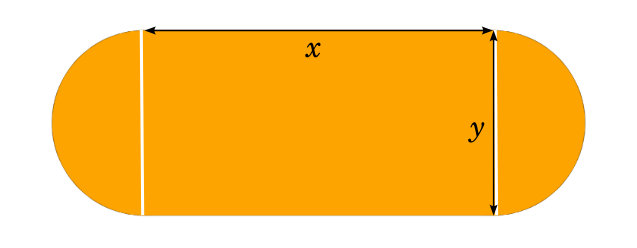
\includegraphics[width=8cm,height=3cm]{img/examen-2022-12-21/pildora.png}

Si el contenido de las píldoras debe ser de \(0.15\) ml, hallar las
dimensiones de \(x\) e \(y\) para que el material empleado en el
envoltorio sea mínimo.

\end{exercise}

\begin{tcolorbox}[enhanced jigsaw, coltitle=black, colbacktitle=quarto-callout-tip-color!10!white, bottomtitle=1mm, opacitybacktitle=0.6, breakable, bottomrule=.15mm, colframe=quarto-callout-tip-color-frame, toprule=.15mm, titlerule=0mm, arc=.35mm, colback=white, title=\textcolor{quarto-callout-tip-color}{\faLightbulb}\hspace{0.5em}{Solución}, leftrule=.75mm, rightrule=.15mm, opacityback=0, left=2mm, toptitle=1mm]

El volumen de una esfera de radio \(r\) es \(v_e(r)=\frac{4}{3}\pi r^3\)
y el de un cilindro de radio \(r\) y altura \(h\) es
\(v_c(r,h)=\pi r^2 h\), de modo que que el volumen de la píldora es
\(v(r,h)=v_e(r)+v_c(r,h) = \frac{4}{3}\pi r^3 + \pi r^2 h\). Como el
volumen de la píldora debe ser \(0.15\) ml \(=0.15\) cm\(^3\),
imponiendo esta restricción, se tiene

\begin{equation}\protect\hypertarget{eq-cont-01-gen-eq1}{}{
v(r,h)=\frac{4}{3}\pi r^3 + \pi r^2 h = 0.15 \Leftrightarrow h = \frac{0.15-\frac{4}{3}\pi r^3}{\pi r^2}.
}\label{eq-cont-01-gen-eq1}\end{equation}

Por otro lado, la superficie de una esfera de radio \(r\) es
\(s_e(r)=4\pi r^2\) y la superficie del envolvente de un cilindro de
radio \(r\) y altura \(h\) es, en realidad, la superficie de un
rectángulo de lados \(2\pi r\) y \(h\), es decir,
\(s_c(r,h) = 2\pi r h\), de manera que la superficie de la píldora es
\(s(r,h) = 4\pi r^2+2\pi r h\), pero sustituyendo el valor de \(h\) que
hemos obtenido de imponer la restricción del volumen se tiene,

\begin{align*}
s(r) &= 4\pi r^2 + 2\pi r \left(\frac{0.15-\frac{4}{3}\pi r^3}{\pi r^2}\right) = 4\pi r^2 + \left(\frac{0.3-\frac{8}{3}\pi r^3}{r}\right)\\ 
&= 4\pi r^2 + \frac{0.3}{r} - \frac{8}{3}\pi r^2 = \frac{4}{3}\pi r^2+ \frac{0.3}{r},
\end{align*}

que es la función a optimizar.

Para calcular el mínimo de la función, calculamos primero los puntos
críticos.

\[
s'(r) = \frac{4}{3}\pi 2r -\frac{0.3}{r^2} =0 \Leftrightarrow \frac{8}{3}\pi r = \frac{0.3}{r^2} \Leftrightarrow r^3 = \frac{0.9}{8\pi} \Leftrightarrow r = \sqrt[3]{\frac{0.9}{8\pi}} \approx 0.3296 \mbox{cm}.
\]

Para ver si en este punto hay un mínimo aplicamos el
\href{https://aprendeconalf.es/analisis-manual/derivadas.html\#thm-concavidad}{criterio
de la segunda derivada}.

\[
s''(r) = \frac{8}{3}\pi -\frac{0.3(-2)}{r^3} =\frac{8}{3}\pi+\frac{0.6}{r^3} >0\ \forall r>0.
\]

Por tanto, \(s\) tiene un mínimo local en \(r=0.3296\), y la altura del
la píldora con la mínima superficie será, utilizando la
Ecuación~\ref{eq-cont-01-gen-eq1},

\[h =\frac{0.15-\frac{4}{3}\pi 0.3296^3}{\pi 0.3296^2}\approx 0.\]

Así pues, las dimensiones óptimas serían \(x=h=0\) cm e \(y=2r=0.6592\)
cm, que en realidad es una esfera de diámetro \(0.6592\) cm.

\end{tcolorbox}

\begin{exercise}[]\protect\hypertarget{exr-9}{}\label{exr-9}

Demostrar que la función
\(f(x)=\ln\left(k\left(x^2-2x+\frac{3}{2}\right)\right)\) no puede tener
más de una raíz en el intervalo \((0,1)\) para cualquier valor de \(k\).

\end{exercise}

\begin{tcolorbox}[enhanced jigsaw, coltitle=black, colbacktitle=quarto-callout-tip-color!10!white, bottomtitle=1mm, opacitybacktitle=0.6, breakable, bottomrule=.15mm, colframe=quarto-callout-tip-color-frame, toprule=.15mm, titlerule=0mm, arc=.35mm, colback=white, title=\textcolor{quarto-callout-tip-color}{\faLightbulb}\hspace{0.5em}{Solución}, leftrule=.75mm, rightrule=.15mm, opacityback=0, left=2mm, toptitle=1mm]

\(x^2-2x+\frac{3}{2}>0\) \(\forall x\in\mathbb{R}\), de manera que, para
que exista la función \(f\), debe ser también \(k>0\) y, por tanto,
aplicando propiedades de logaritmos se tiene,
\(f(x)=\ln\left(k\left(x^2-2x+\frac{3}{2}\right)\right)= \ln(k)+\ln\left(x^2-2x+\frac{3}{2}\right)\).

Por otro lado, como \(x^2-2x+\frac{3}{2}\) es un polinomio, es continuo
en todo \(\mathbb{R}\), y por tanto, \(f(x)\) también es continua en
todo \(\mathbb{R}\), siempre que \(k>0\).

Demostraremos que \(f\) no puede tener más de una raíz en el intervalo
\((0,1)\) por reducción al absurdo. Supongamos que existen
\(0 < a < b < 1\) tales que \(f(a)=f(b)=0\). Entonces, aplicando el
\href{https://aprendeconalf.es/analisis-manual/derivadas.html\#thm-rolle}{teorema
de Rolle}, debe existir algún valor \(c\in(a,b)\) tal que \(f'(c)=0\).
Si calculamos los puntos críticos de \(f\) se tiene

\[
f'(x) = \frac{2x-2}{x^2-2x+3/2} = 0 \Leftrightarrow 2x-2=0 \Leftrightarrow x=1,
\]

pero como \(1\not \in (a,b)\), llegamos a una contradicción ya que no
existe ningún valor \(c\in(a,b)\) con \(f'(c)=0\). Así pues, \(f\) no
puede tener más de una raíz en el intervalo \((0,1)\).

\end{tcolorbox}

\begin{exercise}[]\protect\hypertarget{exr-10}{}\label{exr-10}

Calcular las ecuaciones de las rectas tangente y normal a la gráfica de
la curva implícita \(e^{x^2y}-\ln(\sqrt{x-y})= 0\) en el punto \(x=0\).

\end{exercise}

\begin{tcolorbox}[enhanced jigsaw, coltitle=black, colbacktitle=quarto-callout-tip-color!10!white, bottomtitle=1mm, opacitybacktitle=0.6, breakable, bottomrule=.15mm, colframe=quarto-callout-tip-color-frame, toprule=.15mm, titlerule=0mm, arc=.35mm, colback=white, title=\textcolor{quarto-callout-tip-color}{\faLightbulb}\hspace{0.5em}{Solución}, leftrule=.75mm, rightrule=.15mm, opacityback=0, left=2mm, toptitle=1mm]

En primer lugar obtenemos los valores de \(y\) que cumplen la ecuación
de la curva implícita para \(x=0\). Sustituyendo en la ecuación se tiene

\[\begin{gathered} e^{0^2y}-\ln(\sqrt{0-y})= 0 \Leftrightarrow 1-\ln(\sqrt{-y}) = 0 \Leftrightarrow \\
\ln(\sqrt{-y}) = 1 \Leftrightarrow  \sqrt{-y} = e \Leftrightarrow y=-e^2. \end{gathered}\]

Así pues, hay que calcular la ecuación de las rectas tangente y normal
en el punto \((0,-e^2)\).

Como la pendiente de la recta tangente es la tasa de variación
instantánea, calculamos \(y'=\frac{dy}{dx}\) implícitamente

\[\begin{gathered} \left(e^{x^2y}-\ln(\sqrt{x-y})\right)'= 0' \Leftrightarrow \left(e^{x^2y}-\frac{1}{2}\ln(x-y)\right)'= 0 \Leftrightarrow \\
e^{x^2y}(2xy+x^2y')-\frac{1}{2}\frac{1-y'}{x-y} = 0. \end{gathered}\]

Sustituyendo en \(x=0\) y \(y=-e^2\), se tiene

\[\begin{gathered} e^{0^2(-e^2)}(2\cdot0(-e^2)+0^2y')-\frac{1}{2}\frac{1-y'}{0-(-e^2)} = 0 \\
\Leftrightarrow \frac{-(1-y')}{2e^2} =0 \Leftrightarrow 1-y' = 0 \Leftrightarrow y'=1. \end{gathered}\]

Por tanto, la ecuación de la recta tangente a la curva en \((0,-e^2)\)
es

\[y = y_0 + \frac{dy}{dx}(x_0,y_0) (x-x_0) = (-e^2)+1(x-0) = x-e^2.\]

Y la ecuación de la recta normal a la curva en \((0,-e^2)\) es

\[y = y_0 - \frac{1}{\frac{dy}{dx}(x_0,y_0)} (x-x_0) = (-e^2)-1(x-0) = -x-e^2.\]

\end{tcolorbox}

\bookmarksetup{startatroot}

\hypertarget{examen-de-anuxe1lisis-ii}{%
\chapter{\texorpdfstring{2023-03-11 Examen de Análisis
II}{2023-03-11  Examen de Análisis II}}\label{examen-de-anuxe1lisis-ii}}

\begin{exercise}[]\protect\hypertarget{exr-1}{}\label{exr-1}

Estudiar la convergencia de las siguientes series

\begin{enumerate}
\def\labelenumi{\alph{enumi}.}
\item
  \(\displaystyle \sum \frac{3n^2+2n}{\sqrt{n^5+n}}\)
\item
  \(\displaystyle \sum \cos(n\pi)n^2e^{-n}\)
\end{enumerate}

\end{exercise}

\begin{tcolorbox}[enhanced jigsaw, coltitle=black, colbacktitle=quarto-callout-tip-color!10!white, bottomtitle=1mm, opacitybacktitle=0.6, breakable, bottomrule=.15mm, colframe=quarto-callout-tip-color-frame, toprule=.15mm, titlerule=0mm, arc=.35mm, colback=white, title=\textcolor{quarto-callout-tip-color}{\faLightbulb}\hspace{0.5em}{Solución}, leftrule=.75mm, rightrule=.15mm, opacityback=0, left=2mm, toptitle=1mm]

\begin{enumerate}
\def\labelenumi{\alph{enumi}.}
\item
  Se trata de una serie de términos positivos en la que el término
  dominante en el numerador es \(3n^2\) y el término dominante en el
  denominador es \(n^{5/2}\), por lo que podemos utilizar el
  \href{https://aprendeconalf.es/analisis-manual/08-series.html\#thm-criterio-cociente}{criterio
  del cociente} para compararla con las serie
  \(\sum \frac{3n^2}{n^{5/2}}\).

  \begin{align*}
   \lim_{n\to\infty} \frac{\frac{3n^2+2n}{\sqrt{n^5+n}}}{\frac{3n^2}{n^{5/2}}} 
   &= \lim_{n\to\infty} \frac{3n^2+2n}{3n^2} \frac{\sqrt{n^5+n}}{\sqrt{n^5}} 
   = \lim_{n\to\infty} \frac{3n^2+2n}{3n^2} \lim_{n\to\infty}\frac{\sqrt{n^5+n}}{\sqrt{n^5}} = 1
   \end{align*}

  Por tanto, la serie \(\sum \frac{3n^2+2n}{\sqrt{n^5+n}}\) tiene el
  mismo comportamiento que la serie \(\sum \frac{3n^2}{n^{5/2}}\), y
  como \(\sum \frac{3n^2}{n^{5/2}} = 3\sum \frac{1}{n^{1/2}}\) es una
  serie \(p\) con \(p<1\), diverge, por lo que la serie
  \(\sum \frac{3n^2+2n}{\sqrt{n^5+n}}\) también diverge.
\item
  Se trata de una serie alternada ya que
  \(\sum \cos(n\pi)n^2e^{-n} = \sum (-1)^nn^2e^{-n}\) por lo que
  aplicando el
  \href{https://aprendeconalf.es/analisis-manual/08-series.html\#thm-criterio-serie-alternada}{criterio
  de la serie alternada}, como \(n^2 e^{-n}\) es monótona decreciente
  para \(n\geq 2\) y

  \[
   \lim_{n\to\infty} n^2 e^{-x} 
   = \lim_{n\to\infty} \frac{n^2}{e^x} 
   = \lim_{n\to\infty} \frac{2n}{e^x} 
   = \lim_{n\to\infty} \frac{2}{e^x}
   = 0, \tag{L'Hôpital}
   \]

  se concluye que la serie \(\sum \cos(n\pi)n^2e^{-n}\) converge.
\end{enumerate}

\end{tcolorbox}

\begin{exercise}[]\protect\hypertarget{exr-2}{}\label{exr-2}

Un pozo de petróleo produce 200 mil litros de petróleo el primer año de
su explotación, pero cada año que pasa la producción decae un 12\%.
Calcular la cantidad de petróleo extraída tras \(n\) años de actividad.
¿Qué cantidad total de petróleo se extraerá del pozo hasta agotarlo?

\end{exercise}

\begin{tcolorbox}[enhanced jigsaw, coltitle=black, colbacktitle=quarto-callout-tip-color!10!white, bottomtitle=1mm, opacitybacktitle=0.6, breakable, bottomrule=.15mm, colframe=quarto-callout-tip-color-frame, toprule=.15mm, titlerule=0mm, arc=.35mm, colback=white, title=\textcolor{quarto-callout-tip-color}{\faLightbulb}\hspace{0.5em}{Solución}, leftrule=.75mm, rightrule=.15mm, opacityback=0, left=2mm, toptitle=1mm]

La producción anual evoluciona según la sucesión

\begin{align*}
a_1 &= 200\\
a_2 &= a_1(1-0.12) = 200\cdot 0.88\\
a_3 &= a_20.88 = 200\cdot 0.88^2\\
\vdots\\
a_n &= 200\cdot 0.88^{n-1}
\end{align*}

por lo que la producción acumulada viene dada por la serie
\(\sum 200\cdot 0.88^{n-1}\) que es una serie geométrica de razón
\(0.88\). Así pues, la cantidad de petróleo extraída tras \(n\) años es

\[
A_n = \sum_{i=0}^{n-1} 200\cdot 0.88^i = 200 \frac{1-0.88^n}{1-0.88},
\]

y la cantidad total de petróleo que se extraerá del pozo hasta agotarlo
viene dada por la suma

\[
\sum_{n=0}^\infty 200\cdot 0.88^n = \frac{200}{1-0.88} \approx 1666.6667 \mbox{ mil litros}.
\]

\end{tcolorbox}

\begin{exercise}[]\protect\hypertarget{exr-3}{}\label{exr-3}

Determinar el dominio de convergencia puntual de la serie de potencias

\[
\sum \frac{n(x-3)^n}{(n+1)4^n}
\]

\end{exercise}

\begin{tcolorbox}[enhanced jigsaw, coltitle=black, colbacktitle=quarto-callout-tip-color!10!white, bottomtitle=1mm, opacitybacktitle=0.6, breakable, bottomrule=.15mm, colframe=quarto-callout-tip-color-frame, toprule=.15mm, titlerule=0mm, arc=.35mm, colback=white, title=\textcolor{quarto-callout-tip-color}{\faLightbulb}\hspace{0.5em}{Solución}, leftrule=.75mm, rightrule=.15mm, opacityback=0, left=2mm, toptitle=1mm]

Para determinar el radio de convergencia de la serie de potencias
podemos usar el
\href{https://aprendeconalf.es/analisis-manual/08-series.html\#thm-radio-convergencia-raiz}{criterio
de la raíz}, que establece que

\[
R = \frac{1}{\lim_{n\to\infty} \sqrt[n]{|c_n|}}
\]

Como

\begin{align*}
\lim_{n\to\infty} \sqrt[n]{|c_n|} = \lim_{n\to\infty} \sqrt[n]{\frac{n}{(n+1)4^n}} = \lim_{n\to\infty} \frac{1}{4} \sqrt[n]{\frac{n}{(n+1)}} = \frac{1}{4},
\end{align*}

se concluye que \(R = \frac{1}{1/4} = 4\), de manera que la serie
converge para \(|x-3|<4\), es decir, en el intervalo \((-1,7)\).

Veamos ahora si la serie converge en los extremos del intervalo.

En \(x=7\) se tiene la serie
\(\sum \frac{n4^n}{(n+1)4^n} = \sum \frac{n}{n+1}\), que diverge al ser
\(\lim_{n\to\infty} \frac{n}{n+1} = 1 \neq 0\).

Y en \(x=-1\) se tiene la serie
\(\sum \frac{n(-4)^n}{(n+1)4^n} = \sum (-1)^n\frac{n}{n+1}\), que es una
serie alternada, pero también diverge al ser
\(\left(\frac{n}{n+1}\right)_{n=1}^\infty\) una sucesión monótona
creciente.

Por tanto, el dominio de convergencia puntual de la serie de potencias
es \(\mathcal{C}=(-1,7)\).

\end{tcolorbox}

\begin{exercise}[]\protect\hypertarget{exr-4}{}\label{exr-4}

Calcular la serie de Taylor de la función \(f(x)=\frac{1}{x}\) en
\(a=1\). ¿Cuál es su dominio de convergencia puntual?

\end{exercise}

\begin{tcolorbox}[enhanced jigsaw, coltitle=black, colbacktitle=quarto-callout-tip-color!10!white, bottomtitle=1mm, opacitybacktitle=0.6, breakable, bottomrule=.15mm, colframe=quarto-callout-tip-color-frame, toprule=.15mm, titlerule=0mm, arc=.35mm, colback=white, title=\textcolor{quarto-callout-tip-color}{\faLightbulb}\hspace{0.5em}{Solución}, leftrule=.75mm, rightrule=.15mm, opacityback=0, left=2mm, toptitle=1mm]

Calculamos las primeras derivadas para obtener la expresión de la
derivada de orden \(n\).

\begin{align*}
f(x) &= \frac{1}{x} = x^{-1} & f(1) &= 1^{-1} = 1,\\
f'(x) &= (-1)x^{-2} & f'(1) &= (-1)1^{-2} = -1,\\
f''(x) &= 2x^{-3} & f''(1) &= 2\cdot 1^{-3} = 2,\\
f'''(x) &= (-1)3!x^{-4} & f'''(1) &= (-1)3! 1^{-4} = -3!,\\
\vdots
f^{(n)}(x) &= (-1)^{n+1}n!x^{-(n+1)} & f^{(n)}(1) &= (-1)^{n+1}n!
\end{align*}

Así pues, sustituyendo en la
\href{https://aprendeconalf.es/analisis-manual/08-series.html\#def-serie-taylor}{fórmula
de la serie de Taylor} se obtiene la serie

\[
\sum \frac{f^{n}(1)}{n!}(x-1)^n = \sum \frac{(-1)^{n+1}n!}{n!}(x-1)^n = \sum (-1)^{n+1}(x-1)^n.
\]

Su radio de convergencia puntual se obtiene fácilmente mediante el
criterio de la razón

\[
R = \lim_{n\to\infty} \left|\frac{c_n}{c_{n+1}}\right| = \lim_{n\to\infty} \left|\frac{(-1)^{n+1}}{(-1)^{n+2}}\right| = 1,
\]

por lo que la serie converge en \(|x-1|<1\), es decir, en el intervalo
\((0,2)\). Veamos ahora si converge en los extremos.

En \(x=0\) se tiene la serie
\(\sum (-1)^{n+1}(-1)^n = \sum (-1)^{2n+1} = \sum -1\) que diverge,
mientras que en \(x=2\) se tiene la serie
\(\sum (-1)^{n+1}1^n = \sum (-1)^{n+1}\) que también diverge ya que no
existe el límite \(\lim_{n\to\infty} (-1)^{n+1}\).

Así pues, se concluye que el dominio de convergencia puntual de la serie
de Taylor es \(\mathcal{C}=(0,2)\).

\end{tcolorbox}

\begin{exercise}[]\protect\hypertarget{exr-5}{}\label{exr-5}

Calcular la integral superior de Riemann de la función \(f(x)=2x^3+3x\)
en el intervalo \([0,2]\).

\end{exercise}

\begin{tcolorbox}[enhanced jigsaw, coltitle=black, colbacktitle=quarto-callout-tip-color!10!white, bottomtitle=1mm, opacitybacktitle=0.6, breakable, bottomrule=.15mm, colframe=quarto-callout-tip-color-frame, toprule=.15mm, titlerule=0mm, arc=.35mm, colback=white, title=\textcolor{quarto-callout-tip-color}{\faLightbulb}\hspace{0.5em}{Solución}, leftrule=.75mm, rightrule=.15mm, opacityback=0, left=2mm, toptitle=1mm]

Si dividimos el intervalo \([0,2]\) en \(n\) subintervalos de igual
amplitud, obtenemos la partición \(P_n=\{x_0=0,x_1,\ldots,x_n=2\}\) con
\(x_i=\frac{2i}{n}\) para \(i=1,\ldots,n\).

Como la función \(f(x)=2x^3+3x\) es creciente en el intervalo \([0,2]\)
el máximo de \(f\) en cada subintervalo \((x_{i-1},x_i)\) se alcanzará
en el extremo superior, de manera que la suma superior de Riemann de
\(f\) respecto de \(P_n\) es

\begin{align*}
S(f,P_n) 
&= \sum_{i=1}^n f(x_i)(x_i-x_{i-1}) 
=  \sum_{i=1}^n \left(2\left(\frac{2i}{n}\right)^3 + 3\frac{2i}{n}\right) \frac{2}{n} \\
&= \sum_{i=1}^n \left(\frac{16i^3}{n^3} + \frac{6i}{n}\right) \frac{2}{n} 
= \frac{32}{n^4}\sum_{i=1}^n i^3 + \frac{12}{n^2} \sum_{i=1}^n i \\
&= \frac{32}{n^4}\left(\frac{n(n+1)}{2}\right)^2 + \frac{12}{n^2} \frac{n(n+1)}{2} =  \frac{32}{n^4}\frac{n^4+2n^3+n^2}{4} + 6 \frac{n+1}{n} \\
&= 8\frac{n^4+2n^3+n^2}{n^4} + 6 \frac{n+1}{n}.
\end{align*}

Así pues, la integral superior de Riemann es

\begin{align*}
\overline{\int_0^2}f 
&= \lim_{n\to\infty} S(f,P_n) 
= \lim_{n\to\infty} 8\frac{n^4+2n^3+n^2}{n^4} + 6 \frac{n+1}{n} \\
&= 8 \lim_{n\to\infty} \frac{n^4+2n^3+n^2}{n^4} + 6 \lim_{n\to\infty}\frac{n+1}{n} 
= 8 + 6 = 14.
\end{align*}

\end{tcolorbox}

\bookmarksetup{startatroot}

\hypertarget{examen-de-anuxe1lisis-ii-1}{%
\chapter{\texorpdfstring{2023-06-01 Examen de Análisis
II}{2023-06-01  Examen de Análisis II}}\label{examen-de-anuxe1lisis-ii-1}}

\hypertarget{primera-parte-1}{%
\section{Primera parte}\label{primera-parte-1}}

\begin{exercise}[]\protect\hypertarget{exr-1}{}\label{exr-1}

Calcular las siguientes sumas si existen

\begin{enumerate}
\def\labelenumi{\alph{enumi}.}
\item
  \(\displaystyle \sum_{n=2}^\infty \frac{2}{n^2-1}\).
\item
  \(\displaystyle\sum_{n=1}^\infty (-1)^n \frac{\sqrt{n}}{\ln(n)}\).
\end{enumerate}

\end{exercise}

\begin{tcolorbox}[enhanced jigsaw, coltitle=black, colbacktitle=quarto-callout-tip-color!10!white, bottomtitle=1mm, opacitybacktitle=0.6, breakable, bottomrule=.15mm, colframe=quarto-callout-tip-color-frame, toprule=.15mm, titlerule=0mm, arc=.35mm, colback=white, title=\textcolor{quarto-callout-tip-color}{\faLightbulb}\hspace{0.5em}{Solución}, leftrule=.75mm, rightrule=.15mm, opacityback=0, left=2mm, toptitle=1mm]

\begin{enumerate}
\def\labelenumi{\alph{enumi}.}
\item
  \(\displaystyle \sum_{n=2}^\infty \frac{2}{n^2-1}\) es una serie \(p\)
  con \(p>1\) por lo que la serie converge, pero para calcular su suma
  vamos a reescribir el término general como suma de fracciones simples.

  \[
  \sum_{n=2}^\infty \frac{2}{n^2-1} 
  = \sum_{n=2}^\infty \frac{2}{(n+1)(n-1)} 
  = \sum_{n=2}^\infty \frac{1}{n-1}-\frac{1}{n+1},
  \]

  que es una serie telescópica, de manera que

  \[
  \sum_{n=2}^\infty \frac{2}{n^2-1} = 1 +\frac{1}{2}+ \lim_{n\to\infty}\frac{2}{n^2-1} = \frac{3}{2}.
  \]
\item
  \(\displaystyle\sum_{n=1}^\infty (-1)^n \frac{\sqrt{n}}{\ln(n)}\) es
  una serie alternada, pero

  \begin{align*}
   \lim_{n\to\infty} \frac{\sqrt{n}}{\ln(n)} 
   &= \lim_{n\to\infty} \frac{\frac{1}{2\sqrt{n}}}{\frac{1}{n}} \tag{L'Hôpital}\\
   &= \lim_{n\to\infty} \frac{n}{2\sqrt{n}} 
   = \infty,
   \end{align*}

  por lo que la serie diverge.
\end{enumerate}

\end{tcolorbox}

\begin{exercise}[]\protect\hypertarget{exr-2}{}\label{exr-2}

Considérese el conjunto de Cantor que resulta de ir eliminando del
intervalo \([0,10]\), de manera recursiva, el \(80\%\) central de los
intervalos restantes. El procedimiento sería el siguiente:

\begin{itemize}
\tightlist
\item
  Etapa 1: Se elimina el intervalo \((1,9)\).
\item
  Etapa 2: Se eliminan los intervalos \((0.1,0.9)\) y \((9.1,9.9)\).
\item
  Etapa 3: Se eliminan los intervalos \((0.01,0.09)\), \((0.91,0.99)\),
  \((9.01,9.09)\) y \((9.91,9.99)\).
\item
  \ldots{}
\end{itemize}

¿Cuál es la longitud total de los intervalos eliminados?

\end{exercise}

\begin{tcolorbox}[enhanced jigsaw, coltitle=black, colbacktitle=quarto-callout-tip-color!10!white, bottomtitle=1mm, opacitybacktitle=0.6, breakable, bottomrule=.15mm, colframe=quarto-callout-tip-color-frame, toprule=.15mm, titlerule=0mm, arc=.35mm, colback=white, title=\textcolor{quarto-callout-tip-color}{\faLightbulb}\hspace{0.5em}{Solución}, leftrule=.75mm, rightrule=.15mm, opacityback=0, left=2mm, toptitle=1mm]

En la primera etapa se elimina el intervalo \((1,9)\), que tiene
longitud \(8\). En la segunda etapa se eliminan \(2\) intervalos,
\((0.1,0.9)\) y \((9.1,9.9)\), ambos con amplitud \(0.8\), y por tanto,
la longitud de los intervalos eliminados es \(2\cdot 0.8\). En la
tercera etapa se eliminan \(4\) intervalos, \((0.01,0.09)\),
\((0.91,0.99)\), \((9.01,9.09)\) y \((9.91,9.99)\), ambos con amplitud
\(0.08\), y por tanto, la longitud de los intervalos eliminados es
\(4\cdot 0.08\). En general, en la etapa \(n\) se eliminan \(2^{n-1}\)
intervalos, todos con amplitud \(\frac{8}{10^{n-1}}\), y por tanto, la
longitud de los intervalos eliminados es \(2^{n-1}\frac{8}{10^{n-1}}\).
Así pues, la suma de las longitudes de los intervalos eliminados viene
dada por la serie

\[
\sum_{n=1}^\infty 2^{n-1}\frac{8}{10^{n-1}} 
= \sum_{n=0}^\infty 2^n\frac{8}{10^n} 
= 8\sum_{n=0}^\infty \left(\frac{2}{10}\right)^n,
\]

que es una serie geométrica de razón \(\frac{2}{10}<1\), por lo que que
converge y su suma vale

\[
8\sum_{n=0}^\infty \left(\frac{2}{10}\right)^n 
= 8 \frac{1}{1-\frac{2}{10}} 
= 8 \frac{10}{8} 
= 10.
\]

\end{tcolorbox}

\begin{exercise}[]\protect\hypertarget{exr-3}{}\label{exr-3}

La distribución de Borel de parámetro \(\mu\geq 0\) es una distribución
de probabilidad discreta con recorrido \(\mathbb{N}\) y función de
probabilidad ñ \[
f(n) = \frac{(\mu n)^{n-1}}{e^{\mu n}n!}\ \forall n\in\mathbb{N}, 
\]

¿Para qué valores de \(\mu\) la serie \(\sum f(n)\) es absolutamente
convergente?

\end{exercise}

\begin{tcolorbox}[enhanced jigsaw, coltitle=black, colbacktitle=quarto-callout-tip-color!10!white, bottomtitle=1mm, opacitybacktitle=0.6, breakable, bottomrule=.15mm, colframe=quarto-callout-tip-color-frame, toprule=.15mm, titlerule=0mm, arc=.35mm, colback=white, title=\textcolor{quarto-callout-tip-color}{\faLightbulb}\hspace{0.5em}{Solución}, leftrule=.75mm, rightrule=.15mm, opacityback=0, left=2mm, toptitle=1mm]

Para estudiar la convergencia absoluta de la serie
\(\sum_{n=1}^\infty \frac{(\mu n)^{n-1}}{e^{\mu n}n!}\), aplicamos el
criterio de la razón.

\begin{align*}
\lim_{n\to\infty} \left|\frac{a_{n+1}}{a_n}\right| 
&= \lim_{n\to\infty} \frac{\frac{(\mu(n+1))^n}{e^{\mu(n+1)}(n+1)!}}{\frac{(\mu n)^{n-1}}{e^{\mu n}n!}}
= \lim_{n\to\infty} \frac{\mu^n (n+1)^n e^{\mu n}n!}{\mu^{n-1}n^{n-1}e^{\mu(n+1)}(n+1)!} \\
&= \lim_{n\to\infty} \frac{\mu (n+1)(n+1)^{n-1} e^{\mu n}n!}{n^{n-1}e^{\mu}e^{\mu n}(n+1)n!} 
= \lim_{n\to\infty} \frac{\mu}{e^\mu}\left(\frac{n+1}{n}\right)^{n-1}\\
&= \frac{\mu}{e^\mu}\lim_{n\to\infty} \left(1+\frac{1}{n}\right)^{n-1} 
= \frac{\mu}{e^\mu} e 
= \frac{\mu}{e^{\mu-1}}. 
\end{align*}

Como \(\frac{mu}{e^{\mu-1}} < 1 \Leftrightarrow \mu < e^{\mu-1}\), es
cierto para cualquier \(\mu\geq 0\) excepto para \(\mu=1\), la serie
converge absolutamente \(\forall \mu\geq 0\), \(\mu\neq 1\). Para
\(\mu=1\) el criterio de la razón no es concluyente.

\end{tcolorbox}

\begin{exercise}[]\protect\hypertarget{exr-4}{}\label{exr-4}

Calcular la integral inferior de Riemann de la parábola \(f(x)=3x^2+2x\)
en el intervalo \([0,10]\).

\end{exercise}

\begin{tcolorbox}[enhanced jigsaw, coltitle=black, colbacktitle=quarto-callout-tip-color!10!white, bottomtitle=1mm, opacitybacktitle=0.6, breakable, bottomrule=.15mm, colframe=quarto-callout-tip-color-frame, toprule=.15mm, titlerule=0mm, arc=.35mm, colback=white, title=\textcolor{quarto-callout-tip-color}{\faLightbulb}\hspace{0.5em}{Solución}, leftrule=.75mm, rightrule=.15mm, opacityback=0, left=2mm, toptitle=1mm]

Si dividimos el intervalo \([0,1]\) en \(n\) subintervalos de igual
amplitud obtenemos la partición \(P_n=\{x_0=0, x_1,\ldots, x_n=10\}\)
con \(x_i=\frac{10i}{n}\) \(\forall i=1,\ldots, n\). Como la función
\(f(x)=3x^2+2x\) es creciente en el intervalo \([0,10]\), el mínimo de
\(f\) en cada subintervalo \([x_{i-1},x_i]\) se alcanzará en el extremo
inferior, de manera que la suma inferior de Riemann de \(f\) con
respecto a \(P_n\) es

\begin{align*}
s(f,P_n) 
&= \sum_{i=1}^n f(x_{i-1})(x_i-x_{i-1}) \\
&= \sum_{i=1}^n \left(3\left(\frac{10(i-1)}{n}\right)^2 + 2\left(\frac{10(i-1)}{n}\right)\right)\frac{10}{n} \\
&= \frac{10}{n}\left(\sum_{i=1}^n \frac{300}{n^2}(i-1)^2 + \sum_{i=1}^n \frac{20}{n} (i-1)\right) \\
&= \frac{3000}{n^3} \sum_{i=1}^n (i-1)^2 + \frac{200}{n^2} \sum_{i=1}^n (i-1) \\
&= \frac{3000}{n^3} \sum_{i=1}^n i^2+2i+1 + \frac{200}{n^2} \sum_{i=1}^n (i-1) \\
&= \frac{3000}{n^3} \left(\sum_{i=1}^n i^2 - 2\sum_{i=1}^n i + \sum_{i=1}^n 1\right) + \frac{200}{n^2} \left(\sum_{i=1}^n i - \sum_{i=1}^n 1\right) \\
&= \frac{3000}{n^3} \left(\frac{n(n+1)(2n+1)}{6} -2 \frac{n(n+1)}{2} + n\right) + \frac{200}{n^2} \left(\frac{n(n+1)}{2} -n\right) \\
&= \frac{3000}{n^3} \left(\frac{n^3}{3}+\frac{n^2}{2}+\frac{n}{6}-n^2-n+n\right) + \frac{200}{n^2} \left(\frac{n^2}{2}+\frac{n}{2}-n\right) \\
&= 500 \left(\frac{2n^3-3n^2+n}{n^3}\right) + 100 \left(\frac{n^2-n}{n^2}\right).
\end{align*}

Y la integral inferior de Riemann es

\begin{align*}
\underline{\int_0^{10}} f 
&= \lim_{n\to\infty} s(f,P_n) 
= \lim_{n\to\infty} 500 \left(\frac{2n^3-3n^2+n}{n^3}\right) + 100 \left(\frac{n^2-n}{n^2}\right) \\
&= 500  \lim_{n\to\infty} \left(\frac{2n^3-3n^2+n}{n^3}\right) + 100 \lim_{n\to\infty} \left(\frac{n^2-n}{n^2}\right) \\
&= 500\cdot 2 + 100 = 1100.
\end{align*}

\end{tcolorbox}

\hypertarget{segunda-parte-1}{%
\section{Segunda parte}\label{segunda-parte-1}}

\begin{exercise}[]\protect\hypertarget{exr-5}{}\label{exr-5}

La función \(f(t)=50\sqrt{t/2}+100\) da los ingresos de una empresa en
miles de euros \(t\) años después de su creación, mientras que la
función \(g(t)=\ln(t^2+1)+100\) da los gastos. Calcular el beneficio
acumulado de la empresa entre el quinto y el décimo año.

\end{exercise}

\begin{tcolorbox}[enhanced jigsaw, coltitle=black, colbacktitle=quarto-callout-tip-color!10!white, bottomtitle=1mm, opacitybacktitle=0.6, breakable, bottomrule=.15mm, colframe=quarto-callout-tip-color-frame, toprule=.15mm, titlerule=0mm, arc=.35mm, colback=white, title=\textcolor{quarto-callout-tip-color}{\faLightbulb}\hspace{0.5em}{Solución}, leftrule=.75mm, rightrule=.15mm, opacityback=0, left=2mm, toptitle=1mm]

Para obtener el beneficio acumulado de la empresa ente el quinto y
décimo año tenemos que calcular la integral definida de la función de
los ingresos menos la de los gastos en el intervalo \([5,10]\), es
decir,

\begin{align*}
\int_5^{10} f(t)-g(t) \,dt 
&= \int_5^{10} 50 \sqrt{t/2} + 100 - \ln(t^2+1)-100\,dt \\
&= \frac{50}{\sqrt{2}}\int_5^{10} t^{1/2} \,dt - \int_5^{10}  \ln(t^2+1)\, dt.
\end{align*}

Vamos a calcular estas dos integrales por separado.

\begin{align*}
\int_5^{10} t^{1/2}\,dt =  \left[\frac{t^{3/2}}{3/2}\right]_0^{10} = \frac{2}{3}(10^{3/2}-5^{3/2}) \approx 13.6283.
\end{align*}

y

\begin{align*}
\int_5^{10}  \ln(t^2+1)\,dt 
&= [t \ln(t^2+1)]_5^{10} - \int_5^{10} t \frac{2t}{t^2+1}\,dt \tag{Partes}\\
&= [t \ln(t^2+1)]_5^{10} - 2\int_5^{10} 1 - \frac{1}{t^2+1}\,dt\\
&=  [t \ln(t^2+1)]_5^{10} - [2t]_5^{10} + [2\operatorname{arctg}(t)]_5^{10} \\
&= 10\ln(10^2+1)-5\ln(5^2+1) -2\cdot 10+2\cdot 5 + 2\operatorname{arctg}(10)- 2\operatorname{arctg}(5) \\
&\approx 20.0562.
\end{align*}

Así pues el beneficio acumulado es

\[
\int_5^{10} f(t)-g(t) \,dt \approx \frac{50}{\sqrt{2}} \cdot 13.6283 - 20.0562  = 461.7768  \mbox{ miles de €}.
\]

\end{tcolorbox}

\begin{exercise}[]\protect\hypertarget{exr-6}{}\label{exr-6}

Calcular el área de región encerrada por la curva polar
\(r=2\cos(\theta)\operatorname{sen}(\theta)\).

\end{exercise}

\begin{tcolorbox}[enhanced jigsaw, coltitle=black, colbacktitle=quarto-callout-tip-color!10!white, bottomtitle=1mm, opacitybacktitle=0.6, breakable, bottomrule=.15mm, colframe=quarto-callout-tip-color-frame, toprule=.15mm, titlerule=0mm, arc=.35mm, colback=white, title=\textcolor{quarto-callout-tip-color}{\faLightbulb}\hspace{0.5em}{Solución}, leftrule=.75mm, rightrule=.15mm, opacityback=0, left=2mm, toptitle=1mm]

La función \(r=2\cos(\theta)\operatorname{sen}(\theta)\) tiene periodo
\(\pi\), pero para describir la curva completa es necesario que
\(\theta\) recorra la circunferencia entera, por lo que el intervalo de
integración es \([0,2\pi]\) y, por tanto, para calcular el
\href{https://aprendeconalf.es/analisis-manual/09-integrales.html\#c\%C3\%A1lculo-del-area-encerrada-por-una-curva-en-coordenadas-polares}{área
encerrada por esta curva polar} tenemos que calcula la siguiente
integral.

\begin{align*}
\int_0^{2\pi} \frac{r^2}{2}\,d\theta 
&= \frac{1}{2}\int_0^{2\pi} 2\cos(\theta)\operatorname{sen}(\theta)\,d\theta \\
&= \frac{1}{2}\int_0^{2\pi} \operatorname{sen}(2\theta)^2\,d\theta 
= \frac{1}{4} \int_0^{4\pi} \operatorname{sen}(x)^2\,dx \tag{Cambio $x=2\theta$}\\
&= \frac{1}{4} \int_0^{4\pi} \frac{1-\cos(2x)}{2}\,dx 
= \frac{1}{8} \int_0^{4\pi}\,dx -\int_0^{4\pi} \cos(2x)\,dx \\
&= \frac{1}{8}\left([x]_0^{4\pi}-\left[\frac{1}{2}\operatorname{sen}(2x)\right]_0^{4\pi}\right) \\
&=\frac{1}{8}4\pi = \frac{\pi}{2}.
\end{align*}

\end{tcolorbox}

\begin{exercise}[]\protect\hypertarget{exr-7}{}\label{exr-7}

Calcular el volumen del depósito generado al rotar alrededor del eje
\(y\) la gráfica de la función \(f(x)=(x-1)^2\) con \(0\leq x\leq 3\).
Plantear la integral para obtener la cantidad de chapa necesaria para su
construcción, sin llegar a calcularla.

\end{exercise}

\begin{tcolorbox}[enhanced jigsaw, coltitle=black, colbacktitle=quarto-callout-tip-color!10!white, bottomtitle=1mm, opacitybacktitle=0.6, breakable, bottomrule=.15mm, colframe=quarto-callout-tip-color-frame, toprule=.15mm, titlerule=0mm, arc=.35mm, colback=white, title=\textcolor{quarto-callout-tip-color}{\faLightbulb}\hspace{0.5em}{Solución}, leftrule=.75mm, rightrule=.15mm, opacityback=0, left=2mm, toptitle=1mm]

Para calcular el volumen del sólido de revolución generado al rotar
alrededor del eje \(y\) la gráfica de la función \(f(x)=(x-1)^2\) en el
intervalo \([0,3]\) utilizaremos
\href{https://aprendeconalf.es/analisis-manual/09-integrales.html\#c\%C3\%A1lculo-de-vol\%C3\%BAmenes-de-s\%C3\%B3lidos-de-revoluci\%C3\%B3n-con-envoltorios-cil\%C3\%ADndricos}{envoltorios
cilíndricos}, de manera que el volumen viene dado por la integral

\begin{align*}
\int_0^3 2\pi xf(x)\,dx
&= 2\pi \int_0^3 x(x-1)^2\,dx 
= 2\pi \int_0^3 x(x^2-2x+1)\,dx \\
&= 2\pi \int_0^3 x^3-2x^2+x\,dx
= 2\pi\left[\frac{x^4}{4}-2\frac{x^3}{3}+\frac{x^2}{2}\right]_0^3 \\
&= 2\pi \left(\frac{3^4}{4}-2\frac{3^3}{3}+\frac{3^2}{2}\right)
= \frac{27\pi}{2} \mbox{unidades$^3$}.
\end{align*}

Por otro lado, la chapa necesaria para su construcción viene dada por la
superficie del sólido de revolución y para calcular el
\href{https://aprendeconalf.es/analisis-manual/09-integrales.html\#c\%C3\%A1lculo-de-superficies-de-s\%C3\%B3lidos-de-revoluci\%C3\%B3n}{área
de la superficie de un sólido de revolución} cuando la gráfica de \(f\)
se rota alrededor del eje \(x\) se utiliza la integral

\[
\int_0^3 2\pi f(x)\sqrt{1+f'(x)^2}\,dx
\]

Sin embargo, como la gráfica de \(f\) se rota alrededor del eje \(y\),
el radio del los troncos de conos que resultan al tomar particiones del
intervalo y aproximaciones de Riemman, en lugar de ser \(y=f(x)\), es
\(x\), por lo que la integral que hay que calcular es

\[
\int_0^3 2\pi x\sqrt{1+f'(x)^2}\,dx = 2\pi\int_0^3 x\sqrt{1+(2(x-1))^2}\,dx.
\]

\end{tcolorbox}

\begin{exercise}[]\protect\hypertarget{exr-8}{}\label{exr-8}

La gran pirámide de Gizeh tiene una altura de \(138\) m y una base
cuadrada de lado \(230\) m. Calcular de manera aproximada el trabajo
realizado en su construcción. Supóngase que la densidad de las piedras
usadas en su construcción es de \(2500\) kg/m\(^3\) y que la aceleración
de la gravedad es \(9.81\) m/s\(^2\).

\end{exercise}

\begin{tcolorbox}[enhanced jigsaw, coltitle=black, colbacktitle=quarto-callout-tip-color!10!white, bottomtitle=1mm, opacitybacktitle=0.6, breakable, bottomrule=.15mm, colframe=quarto-callout-tip-color-frame, toprule=.15mm, titlerule=0mm, arc=.35mm, colback=white, title=\textcolor{quarto-callout-tip-color}{\faLightbulb}\hspace{0.5em}{Solución}, leftrule=.75mm, rightrule=.15mm, opacityback=0, left=2mm, toptitle=1mm]

Supongamos que base de la pirámide está centrada en el origen de
coordenadas del plano \(XZ\). Entonces, la ecuación de la recta en la
que queda inscrito el apotema de la pirámide es
\(y=138-\frac{138}{115}x\) de manera que
\(x=\frac{115}{138}(138-y)=115-\frac{5}{6}y\).

Para calcular el trabajo realizado en la construcción de la pirámide,
calcularemos el trabajo realizado para las secciones transversales de la
pirámide con respecto al eje \(y\), que serán cuadrados de lado \(2x\),
y por tanto tendrán área \[
A_i
= \left(2\left(115-\frac{5}{6}y\right)\right)^2 
= \left(230-\frac{5}{3}y\right)^2
= 52900 -\frac{2300}{3}y +\frac{25}{9}y^2 \mbox{ m$^2$}.
\]

Si la altura de cada una de estas secciones transversales es
\(\Delta y\), su volumen es

\[
V_i = A_i\Delta y = \left(52900 -\frac{2300}{3}y +\frac{25}{9}y^2\right)\Delta y \mbox{ m$^3$}.
\]

A partir del volumen de casa sección transversal podemos calcular su
masa multiplicando por la densidad de la piedra.

\[
M_i = V_i\delta = 2500 \left(52900 -\frac{2300}{3}y +\frac{25}{9}y^2\right)\Delta y \mbox{ kg}.
\]

Así pues, la fuerza necesaria para mover la masa de cada una de estas
secciones transversales es

\[
F_i = M_i g = 9.81\cdot 2500 \left(52900 -\frac{2300}{3}y +\frac{25}{9}y^2\right)\Delta y \mbox{ N},
\]

Finalmente, como cada sección transversal debe elevarse una altura
\(y\), el trabajo realizado al mover la masa correspondiente a la
sección transversal es

\[
W_i = F_i y = 9.81\cdot 2500 y \left(52900 -\frac{2300}{3}y +\frac{25}{9}y^2\right)\Delta y \mbox{ J}.
\]

Así pues, el trabajo total será la suma de los trabajos realizados al
desplazar las infinitas secciones transversales desde la base de la
pirámide hasta su cima, es decir, en el intervalo \(y\in [0,138]\), que
viene dado por la integral

\begin{align*}
W 
&= \int_0^{138} 9.81\cdot 2500 y \left(52900 -\frac{2300}{3}y +\frac{25}{9}y^2\right)\,dy \\
&= 24525 \int_0^{138} 52900y -\frac{2300}{3}y^2 +\frac{25}{9}y^3\,dy \\
&= 24525 \left[52900\frac{y^2}{2} -\frac{2300}{3}\frac{y^3}{3} +\frac{25}{9}\frac{y^4}{4}\right]_0^{138} \\
&= 24525\left(26450 \cdot 138^2 - \frac{2300}{9} 138^3 + \frac{25}{36} 138^4\right) 
\approx 2058930157500 \mbox{ J}.
\end{align*}

\end{tcolorbox}

\bookmarksetup{startatroot}

\hypertarget{examen-de-anuxe1lisis-i-2}{%
\chapter{\texorpdfstring{2023-11-15 Examen de Análisis
I}{2023-11-15  Examen de Análisis I}}\label{examen-de-anuxe1lisis-i-2}}

\begin{exercise}[]\protect\hypertarget{exr-1}{}\label{exr-1}

Sea \((x_n)_{n=1}^\infty\) una sucesión tal que

\[
\lim_{n\to\infty} x_{2n}= \lim_{n\to\infty}x_{2n+1}=l.
\]

Demostrar que \(\lim_{n\to\infty}x_n = l\).

\end{exercise}

\begin{tcolorbox}[enhanced jigsaw, coltitle=black, colbacktitle=quarto-callout-tip-color!10!white, bottomtitle=1mm, opacitybacktitle=0.6, breakable, bottomrule=.15mm, colframe=quarto-callout-tip-color-frame, toprule=.15mm, titlerule=0mm, arc=.35mm, colback=white, title=\textcolor{quarto-callout-tip-color}{\faLightbulb}\hspace{0.5em}{Solución}, leftrule=.75mm, rightrule=.15mm, opacityback=0, left=2mm, toptitle=1mm]

Por la definición de límite, como \(\lim_{n\to\infty} x_{2n}= l\),
\(\forall \varepsilon>0\) \(\exists k_1\in\mathbb{N}\) tal que si
\(2n\geq k_1\) entonces \(|x_{2n}-l|<\varepsilon\).

Del mismo modo, como \(\lim_{n\to\infty} x_{2n+1}= l\),
\(\forall \varepsilon>0\) \(\exists k_2\in\mathbb{N}\) tal que si
\(2n+1\geq k_2\) entonces \(|x_{2n+1}-l|<\varepsilon\).

Tomando ahora \(k=\max\{k_1,k_2\}\), si \(m\geq k\), entonces o \(m\) es
par, o \(m\) es impar. Si \(m\) es par entonces existe
\(n\in\mathbb{N}\) tal que \(m=2n\) y como \(m=2n\geq k\geq k_1\), se
tiene que \(|x_m-l|=|x_{2n}-l|<\varepsilon\). Y si \(m\) es impar
entonces existe \(n\in\mathbb{N}\) tal que \(m=2n+1\) y como
\(m=2n+1\geq k\geq k_2\), se tiene que
\(|x_m-l|=|x_{2n+1}-l|<\varepsilon\). Por tanto,
\(\lim_{n\to\infty}x_n = l\).

\end{tcolorbox}

\begin{exercise}[]\protect\hypertarget{exr-2}{}\label{exr-2}

La cantidad de agua almacenada en un embalse en hectómetros cúbicos
viene dada por la función

\[
h(t) = \frac{10t+\cos(2t)}{4t+2\operatorname{sen}(3t)}
\]

Analizar si la cantidad de agua converge o no a largo plazo.

\end{exercise}

\begin{tcolorbox}[enhanced jigsaw, coltitle=black, colbacktitle=quarto-callout-tip-color!10!white, bottomtitle=1mm, opacitybacktitle=0.6, breakable, bottomrule=.15mm, colframe=quarto-callout-tip-color-frame, toprule=.15mm, titlerule=0mm, arc=.35mm, colback=white, title=\textcolor{quarto-callout-tip-color}{\faLightbulb}\hspace{0.5em}{Solución}, leftrule=.75mm, rightrule=.15mm, opacityback=0, left=2mm, toptitle=1mm]

Como \(-1\leq \operatorname{sen}(3t)\leq 1\) y \(-1\leq \cos(2t)\leq 1\)
\(\forall t\in\mathbb{R}\), en particular, para \(t>1\)se tiene que

\[
\begin{gathered}
0 < 10t-1 \leq 10t+\cos(2t) \leq 10t+1 \\
0 < 4t-2 \leq 4t+2\operatorname{sen}(3t) \leq 4t+2
\end{gathered}
\]

y por tanto

\[
\frac{10t-1}{4t+2} \leq \frac{10t+\cos(2t)}{4t+2\operatorname{sen}(3t)} \leq \frac{10t+1}{4t-2}.
\]

Como además, aplicando álgebra de límites,

\begin{align*}
\lim_{t\to\infty} \frac{10t-1}{4t+2} 
&= \lim_{t\to\infty} \frac{\frac{10t-1}{t}}{\frac{4t+2}{t}}
= \lim_{t\to\infty} \frac{10-\frac{1}{t}}{4+\frac{2}{t}}
= \frac{10}{4}, \\
\lim_{t\to\infty} \frac{10t+1}{4t-2} 
&= \lim_{t\to\infty} \frac{\frac{10t+1}{t}}{\frac{4t-2}{t}}
= \lim_{t\to\infty} \frac{10+\frac{1}{t}}{4-\frac{2}{t}}
= \frac{10}{4},
\end{align*}

por el
\href{https://aprendeconalf.es/analisis-manual/06-limites.html\#thm-compresi\%C3\%B3n-funciones}{teorema
de compresión de funciones}, se tiene que

\[
\lim_{t\to\infty} \frac{10t+\cos(2t)}{4t+2\operatorname{sen}(3t)} = \frac{10}{4}.
\]

Otra forma de verlo sería dividiendo numerador y denominador por \(t\)

\begin{align*}
\lim_{t\to\infty} \frac{10t+\cos(2t)}{4t+2\operatorname{sen}(3t)} 
&= \lim_{t\to\infty} \frac{\frac{10t+\cos(2t)}{t}}{\frac{4t+2\operatorname{sen}(3t)}{t}} 
= \lim_{t\to\infty} \frac{10 + \frac{\cos(2t)}{t}}{4 + \frac{2\operatorname{sen}(3t)}{t}} \\
&= \frac{\lim_{t\to\infty}10 +\lim_{t\to\infty} \frac{\cos(2t)}{t}}{\lim_{t\to\infty}4 + \lim_{t\to\infty}\frac{2\operatorname{sen}(3t)}{t}}.
\end{align*}

Ahora bien, como \(-1\leq \cos(2t)\leq 1\), se tiene que

\[
\frac{-1}{t}\leq \frac{\cos(2t)}{t}\leq \frac{1}{t},
\]

y como
\(\lim_{t\to\infty} \frac{-1}{t} = \lim_{t\to\infty} \frac{1}{t} = 0\),
por el teorema de compresión de funciones se tiene que
\(\lim_{t\to\infty} \frac{\cos(2t)}{t} = 0\).

Del mismo modo se puede probar que
\(\lim_{t\to\infty} \frac{2\operatorname{sen}(3t)}{t} =0\), por lo que
finalmente se tiene que

\[
\lim_{t\to\infty} \frac{10t+\cos(2t)}{4t+2\operatorname{sen}(3t)} 
= \frac{10+0}{4+0} = 2.5.
\]

Así pues, a largo plazo, la cantidad de agua en el embalse converge a
\(2.5\) Hm\(^3\).

\end{tcolorbox}

\begin{exercise}[]\protect\hypertarget{exr-3}{}\label{exr-3}

Dado el conjunto
\(A=\{\frac{\operatorname{sin}(n)}{n}, n\in\mathbb{N}\}\),

\begin{enumerate}
\def\labelenumi{\alph{enumi}.}
\tightlist
\item
  Calcular su ínfimo, mínimo, supremo y máximo si existen.
\item
  Calcular sus puntos de acumulación.
\item
  Estudiar si se trata de un conjunto abierto o cerrado.
\end{enumerate}

\end{exercise}

\begin{tcolorbox}[enhanced jigsaw, coltitle=black, colbacktitle=quarto-callout-tip-color!10!white, bottomtitle=1mm, opacitybacktitle=0.6, breakable, bottomrule=.15mm, colframe=quarto-callout-tip-color-frame, toprule=.15mm, titlerule=0mm, arc=.35mm, colback=white, title=\textcolor{quarto-callout-tip-color}{\faLightbulb}\hspace{0.5em}{Solución}, leftrule=.75mm, rightrule=.15mm, opacityback=0, left=2mm, toptitle=1mm]

\begin{enumerate}
\def\labelenumi{\alph{enumi}.}
\item
  Los elementos del conjunto están más cerca de 0 a medida que \(n\)
  crece, aunque irán alternado el signo, ya que
  \(-1\leq\operatorname{sin}(n)\leq 1\) \(\forall n\in \mathbb{N}\), por
  tanto el conjunto estará acotado tanto inferior como superiormente. Si
  calculamos de manera aproximada los primeros elementos del conjunto
  para \(n=1,\ldots,10\), tenemos

  \[
  \begin{array}{cc}
  \hline
  n &  \frac{\operatorname{sen}(n)}{n} \\
  1 & 0.8415 \\
  2 & 0.4546 \\
  3 & 0.0470 \\
  4 & -0.1892 \\
  5 & -0.1917 \\
  6 & -0.04656 \\
  7 & 0.0938 \\
  \vdots & \vdots \\
  \hline
  \end{array}
  \]

  A partir de aquí los valores se van acercando cada vez más a 0 ya que
  \(\lim{n\to \infty}\frac{\operatorname{sen}(n)}{n} = 0\). Por tanto,
  el máximo valor del \(A\) es el correspondiente a \(n=1\), es decir,
  \(\operatorname{sen}(1)\approx 0.8415\), y el mínimo corresponde a
  \(n=5\), es decir \(\operatorname{sen}(5)/5 \approx -0.1917\). Y como
  el mínimo y el máximo existen, coinciden con el ínfimo y el supremo,
  respectivamente.
\item
  Como los valores del conjunto están cada vez más cerca de \(0\), este
  será un punto de acumulación. Para demostrarlo basta con ver que
  \(\lim{n\to \infty}\frac{\operatorname{sen}(n)}{n} = 0\), ya que, como
  \(-1\leq\operatorname{sin}(x)\leq 1\) \(\forall n\in \mathbb{N}\), se
  tiene que

  \[
  \frac{-1}{n}\leq \frac{\operatorname{sen}(n)}{n}\leq \frac{1}{n}
  \]

  y como
  \(\lim_{n\to\infty} \frac{-1}{n}=\lim_{n\to\infty} \frac{1}{n} = 0\),
  y por el teorema de compresión de sucesiones se tiene que
  \(\lim{n\to \infty}\frac{\operatorname{sen}(n)}{n} = 0\), y por tanto,
  se cumple que \(\forall \varepsilon>0\) existe \(k\in\mathbb{N}\) tal
  que
  \(\left|\frac{\operatorname{sen}(n)}{n} - 0 \right| < \varepsilon\),
  por lo que podemos encontrar puntos de \(A\) tan cerca de \(0\) como
  queramos y \(0\) es un punto de acumulación.

  Veamos ahora que \(0\) es el único punto de acumulación de \(A\), es
  decir, que cualquier otro punto \(x\neq 0\) no es punto de
  acumulación. Supongamos que \(x\neq 0\) es un punto de acumulación de
  \(A\), entonces es posible construir una sucesión de puntos
  \((a_n)_{n=1}^\infty\) tal que \(a_n\in A\) y \(a_n\neq x\)
  \(\forall n\in \mathbb{N}\), que converge a \(x\). Pero, por otro
  lado, como \(\lim{n\to \infty}\frac{\operatorname{sen}(n)}{n} = 0\),
  cualquier subsucesión de la sucesión
  \(\left(\frac{\operatorname{sen}(n)}{n}\right)\) converge a \(0\), y
  en particular la sucesión \((a_n)_{n=1}^\infty\), por lo que
  \(\lim_{n\to\infty} a_n = 0\), lo cual es contradictorio con que
  \(x\neq 0\).
\item
  \(A\) no puede ser cerrado porque \(0\) es un punto de acumulación
  suyo pero \(0\not\in A\) (ver
  \href{https://aprendeconalf.es/analisis-manual/03-topologia-reales.html\#thm-conjunto-cerrado-puntos-acumulacion}{teorema}).
  Pero \(A\) tampoco es abierto porque sus puntos son aislados, es
  decir, para cualquier \(n\in\mathbb{N}\), y \(\forall \varepsilon>0\)
  el intervalo
  \(\left(\frac{\operatorname{sen}(n)}{n}-\varepsilon, \frac{\operatorname{sen}(n)}{n}-\varepsilon\right)\)
  siempre contiene puntos que no son de \(A\).
\end{enumerate}

\end{tcolorbox}

\begin{exercise}[]\protect\hypertarget{exr-4}{}\label{exr-4}

Dada la función \(f(x)=\dfrac{ax^n}{x^2+bx}\),

\begin{enumerate}
\def\labelenumi{\alph{enumi}.}
\tightlist
\item
  ¿Cuánto debe valer \(a\), \(b\) y \(n\) para que \(f\) tenga una
  asíntota vertical \(x=3\) y una asíntota horizontal \(y=2\)?
\item
  ¿Cuánto debe valer \(a\), \(b\) y \(n\) para que \(f\) tenga una
  asíntota oblicua \(y=3x-1\)?
\end{enumerate}

\end{exercise}

\begin{tcolorbox}[enhanced jigsaw, coltitle=black, colbacktitle=quarto-callout-tip-color!10!white, bottomtitle=1mm, opacitybacktitle=0.6, breakable, bottomrule=.15mm, colframe=quarto-callout-tip-color-frame, toprule=.15mm, titlerule=0mm, arc=.35mm, colback=white, title=\textcolor{quarto-callout-tip-color}{\faLightbulb}\hspace{0.5em}{Solución}, leftrule=.75mm, rightrule=.15mm, opacityback=0, left=2mm, toptitle=1mm]

\begin{enumerate}
\def\labelenumi{\alph{enumi}.}
\item
  Para que \(f\) tenga una asíntota vertical en \(x=3\) debe anularse el
  denominador, es decir, \(3^2+3b=0\), de donde se deduce que \(b=-3\),
  ya que

  \begin{align*}
  \lim_{x\to 3^-}\frac{ax^n}{x^2-3x}  
  &= \infty \\
  \lim_{x\to 3^+}\frac{ax^n}{x^2-3x}  
  &= -\infty
  \end{align*}

  Y para que \(f\) tenga una asíntota horizontal \(y=2\), debe ser
  \(\lim_{x\to \pm\infty} \frac{ax^n}{x^2-3x} = 2\), y para ello es
  necesario que el grado del polinomio del numerador sea igual al grado
  del polinomio del denominador, es decir, \(n=2\). En tal caso,

  \[
  \lim_{x\to \pm\infty} \frac{ax^2}{x^2-3x}
  = \lim_{x\to \pm\infty} \frac{\frac{ax^2}{x^2}}{\frac{x^2-3x}{x^2}}
  = \lim_{x\to \pm\infty} \frac{a}{1-\frac{3}{x}} 
  = a,
  \]

  de modo que debe ser \(a=2\).
\item
  Para que \(f\) tenga una asíntota oblicua \(y=3x-1\), debe ser
  \(\lim_{x\to\pm\infty} \frac{f(x)}{x}=3\). Como

  \[
  \lim_{x\to\pm\infty} \frac{\frac{ax^n}{x^2+bx}}{x} 
  = \lim_{x\to\pm\infty} \frac{ax^n}{x^3+bx^2},
  \]

  y para que este límite exista, el grado del polinomio del numerador
  debe ser igual que el del denominador, es decir, \(n=3\), y en tal
  caso se tiene

  \[
  \lim_{x\to\pm\infty} \frac{\frac{ax^3}{x^2+bx}}{x} 
  = \lim_{x\to\pm\infty} \frac{ax^3}{x^3+bx^2}
  = \lim_{x\to\pm\infty} \frac{\frac{ax^3}{x^3}}{\frac{x^3+bx^2}{x^3}}
  = \lim_{x\to\pm\infty} \frac{a}{1+\frac{b}{x}}
  = a,
  \]

  de manera que debe ser \(a=3\).

  Por otro lado, también debe cumplirse que
  \(\lim_{x\to\pm\infty} f(x)-3x = -1\). Como

  \begin{align*}
  \lim_{x\to\pm\infty} \frac{3x^3}{x^2+bx} -3x 
  &= \lim_{x\to\pm\infty} \frac{3x^3-3x^3-3bx^2}{x^2+bx}
  = \lim_{x\to\pm\infty} \frac{\frac{-3bx^2}{x^2}}{\frac{x^2+bx}{x^2}} \\
  &= \lim_{x\to\pm\infty} \frac{-3b}{1+\frac{b}{x}}
  = -3b,
  \end{align*}

  de donde se deduce que \(b=1/3\).
\end{enumerate}

\end{tcolorbox}

\begin{exercise}[]\protect\hypertarget{exr-5}{}\label{exr-5}

La sucesión de Fibonacci se define como

\[
a_1 = a_2 = 1 \quad \mbox{y}\quad a_{n+1} = a_n + a_{n-1}.
\]

Demostrar que la sucesión
\(\left(\dfrac{a_{n+1}}{a_n}\right)_{n=1}^\infty\) converge al número
\(\phi = \frac{1+\sqrt{5}}{2}\).

\end{exercise}

\begin{tcolorbox}[enhanced jigsaw, coltitle=black, colbacktitle=quarto-callout-tip-color!10!white, bottomtitle=1mm, opacitybacktitle=0.6, breakable, bottomrule=.15mm, colframe=quarto-callout-tip-color-frame, toprule=.15mm, titlerule=0mm, arc=.35mm, colback=white, title=\textcolor{quarto-callout-tip-color}{\faLightbulb}\hspace{0.5em}{Solución}, leftrule=.75mm, rightrule=.15mm, opacityback=0, left=2mm, toptitle=1mm]

Sea \(x_n=\frac{a_{n+1}}{a_n}\), donde \((a_n)_{n=1}^\infty\) es la
sucesión de Fibonacci. Entonces

\[
x_{n+1} 
= \frac{a_{n+2}}{a_{n+1}}
= \frac{a_{n+1}+a_n}{a_{n+1}}
= 1 + \frac{a_{n}}{a_{n+1}}
= 1 + \frac{1}{\frac{a_{n+1}}{a_n}}
= 1 + \frac{1}{x_n},
\]

que converge al número \(\phi = \frac{1+\sqrt{5}}{2}\), tal y como se
vió en este
\href{https://aprendeconalf.es/analisis-ejercicios/04-sucesiones.html\#exr-numero-aureo}{ejercicio}.

\end{tcolorbox}

\bookmarksetup{startatroot}

\hypertarget{examen-de-anuxe1lisis-iii}{%
\chapter{\texorpdfstring{2023-11-14 Examen de Análisis
III}{2023-11-14  Examen de Análisis III}}\label{examen-de-anuxe1lisis-iii}}

\begin{exercise}[]\protect\hypertarget{exr-1}{}\label{exr-1}

Una fábrica de componentes electrónicos produce dos tipos de chips. Los
ingresos, en cientos de euros, obtenidos por la venta de \(x\) miles de
unidades del primer tipo e \(y\) miles de unidades del segundo tipo
vienen dados por la función
\(I(x,y) = -x^2-\frac{1}{2}y^2-\frac{1}{4}xy+280x+260y+1000\), mientras
que los gastos de producción, vienen dados por la función
\(C(x,y) = 100x+120y+6000\). ¿Qué cantidad de chips de cada tipo debe
producir la fábrica para maximizar el beneficio?

\end{exercise}

\begin{tcolorbox}[enhanced jigsaw, coltitle=black, colbacktitle=quarto-callout-tip-color!10!white, bottomtitle=1mm, opacitybacktitle=0.6, breakable, bottomrule=.15mm, colframe=quarto-callout-tip-color-frame, toprule=.15mm, titlerule=0mm, arc=.35mm, colback=white, title=\textcolor{quarto-callout-tip-color}{\faLightbulb}\hspace{0.5em}{Solución}, leftrule=.75mm, rightrule=.15mm, opacityback=0, left=2mm, toptitle=1mm]

Si \(I(x,y)\) es la función que da los ingresos y \(C(x,y)\) la que da
los costes, la función que da los beneficios es

\begin{align*}
B(x,y) 
&= -x^2 - \frac{1}{2}y^2 - \frac{1}{4}xy + 280x + 260y + 1000 - (100x + 120y + 6000) \\
&= -x^2 - \frac{1}{2}y^2 - \frac{1}{4}xy + 180x + 140y - 5000.
\end{align*}

Para calcular el máximo de esta función primero hay que obtener los
puntos críticos, es decir, los puntos que anulan las derivadas
parciales.

\begin{align*}
\frac{\partial B}{\partial x} 
&= -2x -\frac{1}{4}y + 180 = 0,\\
\frac{\partial B}{\partial y} 
&= -y -\frac{1}{4}x + 140 = 0.\\
\end{align*}

Resolviendo el sistema de ecuaciones se tiene que la única solución es
el punto \(\left(\frac{2320}{31}, \frac{3760}{31}\right)\).

A continuación, calculamos el hessiano.

\[
|\nabla^2 B(x,y)| =
\begin{vmatrix}
-2 & -\frac{1}{4}\\
-\frac{1}{4} & -1
\end{vmatrix}
= \frac{31}{16},
\]

que es positivo en cualquier punto, y en particular en el punto crítico
\(\left(\frac{2320}{31}, \frac{3760}{31}\right)\), por lo en este punto
hay un extremo relativo, y como
\(\frac{\partial^2 B}{\partial x^2} = -2<0\), se trata de un máximo
relativo. En este punto, el beneficio es

\begin{align*}
B\left(\frac{2320}{31}, \frac{3760}{31}\right) 
&= -\left(\frac{2320}{31}\right)^2 - \frac{1}{2}\left(\frac{3760}{31}\right)^2 - \frac{1}{4}\frac{2320}{31}\frac{3760}{31}  \\
&+ 180 \left(\frac{2320}{31}\right) + 140\left(\frac{3760}{31}\right) - 5000
\approx 10225.81\cdot 10^2 \mbox{€}
\end{align*}

Para ver que es el máximo absoluto, basta con ver que en los límites de
la región del dominio de la función, en este caso
\(\{(x,y), x\geq 0, y\geq 0\}\), no hay ningún punto donde la función
tome un valor mayor. En particular, para \(x=0\) la función de beneficio
es

\[
f(y) = -\frac{1}{2}y^2 + 140y - 5000,
\]

cuyos puntos críticos son

\[
f'(y) = -y + 140 = 0 \Leftrightarrow y = 140.
\]

que es un máximo relativo al ser \(f''(y) = -1<0\), pero
\(f(140) = 4800 < 10225.81\).

Del mismo modo se comprueba que para \(y=0\) tampoco hay valores de
\(x\) donde la función tome un valor mayor que en el máximo relativo.

\end{tcolorbox}

\begin{exercise}[]\protect\hypertarget{exr-2}{}\label{exr-2}

La presión (en Pascales) en la posición \((x,y,z)\) de un espacio es
\(p(x,y,z)= x^2+y^2-z^3\), y la posición de un objeto en cada instante
\(t>0\) (en segundos) en ese mismo espacio está dada por la función
vectorial

\[
\begin{cases}
x=\sqrt{t}\\
y=1\\
z=1/t
\end{cases}
\]

\begin{enumerate}
\def\labelenumi{\alph{enumi}.}
\item
  Calcular la ecuación de la recta tangente a la trayectoria en el punto
  \((1,1,1)\).
\item
  Calcular la ecuación del plano normal a la trayectoria en el punto
  \((1,1,1)\).
\item
  ¿Es la dirección de esta trayectoria al pasar por el punto \((1,1,1)\)
  aquella en la que que el crecimiento de la presión es máximo?
\item
  ¿Cuál es la tasa de variación de la presión que soporta el objeto con
  respecto al tiempo en ese mismo instante?
\end{enumerate}

\end{exercise}

\begin{tcolorbox}[enhanced jigsaw, coltitle=black, colbacktitle=quarto-callout-tip-color!10!white, bottomtitle=1mm, opacitybacktitle=0.6, breakable, bottomrule=.15mm, colframe=quarto-callout-tip-color-frame, toprule=.15mm, titlerule=0mm, arc=.35mm, colback=white, title=\textcolor{quarto-callout-tip-color}{\faLightbulb}\hspace{0.5em}{Solución}, leftrule=.75mm, rightrule=.15mm, opacityback=0, left=2mm, toptitle=1mm]

\begin{enumerate}
\def\labelenumi{\alph{enumi}.}
\item
  Sea \(g(t) = \left(\sqrt{t}, 1, \frac{1}{t}\right)\). Resulta sencillo
  ver que la trayectoria de \(g\) pasa por el punto \((1, 1, 1)\) cuanto
  \(t=1\). Por tanto, se trata de calcular la ecuación de la recta
  tangente a la trayectoria de \(g\) para \(t=1\). La recta tangente la
  trayectoria de \(g\) tiene la dirección que la derivada de la función
  vectorial, que vale
  \(g'(t) = \left(\frac{1}{2\sqrt{t}}, 0, -\frac{1}{t^2}\right)\), y en
  particular, en \(t=1\) vale
  \(g'(1) = \left(\frac{1}{2}, 0, -1\right)\), por lo que la ecuación
  vectorial de la recta tangente resulta ser

  \[
  g(1) + tg'(1) 
  = (1, 1, 1) + t\left(\frac{1}{2}, 0, -1\right)
  = \left(1+\frac{t}{2}, 1, 1-t\right).
  \]
\item
  El plano normal es perpendicular al vector de la derivada, por lo que
  el producto escalar de cualquier vector del plano normal y la derivada
  se anulará, es decir,

  \[
  \begin{gathered}
  ((x, y, z) - g(1)) g'(1) = 0 
  \Leftrightarrow ((x, y, z) - (1, 1, 1)) \left(\frac{1}{2}, 0, -1\right) = 0 \\
  \Leftrightarrow \frac{x-1}{2} -(z-1) = 0
  \Leftrightarrow \frac{x}{2}-z+\frac{1}{2} = 0. 
  \end{gathered}
  \]
\item
  Ya hemos visto que la dirección de la recta tangente a la trayectoria
  de \(g\) es la del vector \(\left(\frac{1}{2}, 0, -1\right)\). Por
  otro lado, la dirección de máximo crecimiento de la \(f\) es la
  dirección del vector gradiente, que vale
  \(\nabla p(x, y, z)= (2x, 2y, -3z^2)\), y en particular en el punto
  \((1, 1, 1,)\) vale \(\nabla f(1, 1, 1) = (2, 2, -3)\). Para que la
  dirección de la recta tangente a la trayectoria de \(g\) sea la misma
  que la dirección de máximo crecimiento de \(p\), ambos vectores
  deberían ser proporcionales, pero no lo son, por lo que ambas
  direcciones son distintas.
\item
  La tasa de variación de la presión con respecto al tiempo es la
  derivada de \(p\circ g\), que, aplicando la regla de la cadena, vale
\end{enumerate}

\[
\frac{dp}{dt} 
= \nabla(1,1,1) g'(1)
= (2, 2, -3) \left(\frac{1}{2},0,-1\right)
= 4 \mbox{ Pa/s}.
\]

\end{tcolorbox}

\begin{exercise}[]\protect\hypertarget{exr-3}{}\label{exr-3}

El consumo de combustible de una avioneta (en l/m) depende de la altura
a la que vuela \(h\) (en km) y su velocidad \(v\) (en cientos de km/h)
según la función \(c(h,v) = \frac{v^2}{\ln(\sqrt{h+2})}\).

\begin{enumerate}
\def\labelenumi{\alph{enumi}.}
\item
  En el momento en que el avión tiene una altitud de 2 km y una
  velocidad de 250 km/h, ¿cómo cambiará el consumo si empezamos a
  cambiar la velocidad y la altura de manera velocidad disminuya la
  mitad de lo que aumenta la altura?
\item
  En ese mismo instante, ¿cómo debería cambiar la altitud y la velocidad
  para que el consumo se reduzca lo más rápidamente posible?
\item
  Si en ese instante, el avión empieza a acelerar a razón de 5 km/h por
  minuto y su altura empieza a disminuir a razón de 100 m por minuto.
  ¿Cuál será la tasa de variación del consumo de combustible con
  respecto al tiempo?
\end{enumerate}

\end{exercise}

\begin{tcolorbox}[enhanced jigsaw, coltitle=black, colbacktitle=quarto-callout-tip-color!10!white, bottomtitle=1mm, opacitybacktitle=0.6, breakable, bottomrule=.15mm, colframe=quarto-callout-tip-color-frame, toprule=.15mm, titlerule=0mm, arc=.35mm, colback=white, title=\textcolor{quarto-callout-tip-color}{\faLightbulb}\hspace{0.5em}{Solución}, leftrule=.75mm, rightrule=.15mm, opacityback=0, left=2mm, toptitle=1mm]

\begin{enumerate}
\def\labelenumi{\alph{enumi}.}
\item
  Para que la velocidad disminuya a razón de la mitad de lo que aumenta
  la altura, debemos cambiar la altura y la velocidad en la dirección
  del vector \((1, -1/2)\). La tasa de variación del consumo la da la
  derivada direccional de \(c\) en esta dirección, y para ello primero
  hay que calcular el vector gradiente. Las derivadas parciales de \(c\)
  son

  \begin{align*}
  \frac{\partial c}{\partial h} 
  &= \frac{-2v^2}{\ln(h+2)^2}\frac{1}{h+2}
  = \frac{-2v^2}{\ln(h+2)^2(h+2)}, \\
  \frac{\partial c}{\partial v} 
  &= \frac{4v}{\ln(h+2)},
  \end{align*}

  por lo que el vector gradiente en el punto \((2, 2.5)\) vale

  \[
  \nabla (2, 2.5) 
  = \left(\frac{-2\cdot 2.5^2}{\ln(2+2)^2(2+2)}, \frac{4\cdot 2.5}{\ln(2+2)}\right)
  = \left(\frac{-3.125}{\ln(4)^2}, \frac{10}{\ln(4)}\right).
  \]

  Así pues, la derivada direccional de \(c\) en la dirección del vector
  \(\mathbf{u}=(1, -1/2)\) es

  \[
  c'_{\mathbf{u}} 
  = \nabla c(2, 2.5) \frac{\mathbf{u}}{|\mathbf{u}|}
  = \left(\frac{-3.125}{\ln(4)^2}, \frac{10}{\ln(4)}\right) \frac{(1, -1/2)}{\sqrt{1^2 + (-1/2)^2}} \approx -4.6804.
  \]
\item
  Para que el consumo se reduzca lo más rápidamente posible, deberíamos
  cambiar la altitud y la velocidad en la dirección opuesta al
  gradiente, es decir, en la dirección del vector
  \(-\nabla c(2,2.5) = \left(\frac{3.125}{\ln(4)^2}, \frac{-10}{\ln(4)}\right)\).
\item
  La tasa de variación del consumo con respecto al tiempo es

  \[
  \frac{dc}{dt} 
  = \nabla c(2, 2.5) \left(\frac{dh}{dt}, \frac{dv}{dt}\right)
  = \left(\frac{3.125}{\ln(4)^2}, \frac{-10}{\ln(4)}\right) (-0.1, 0.05)
  \approx 0.5233 \mbox{ l/min}^2.
  \]
\end{enumerate}

\end{tcolorbox}

\begin{exercise}[]\protect\hypertarget{exr-4}{}\label{exr-4}

Un cable de longitud \(l\) tiene una sección circular de radio \(r\) y
se enrolla sobre un cilindro de radio \(R\). ¿Cuál es la longitud más
corta que debe tener el cilindro para poder enrollar todo el cable sin
que se solape?

Calcular la longitud para un cilindro de radio 10 cm y un cable de 10 m
con una sección circular de radio 2 cm. ¿Cuántas vueltas completas daría
el cable alrededor del cilindro?

\end{exercise}

\begin{tcolorbox}[enhanced jigsaw, coltitle=black, colbacktitle=quarto-callout-tip-color!10!white, bottomtitle=1mm, opacitybacktitle=0.6, breakable, bottomrule=.15mm, colframe=quarto-callout-tip-color-frame, toprule=.15mm, titlerule=0mm, arc=.35mm, colback=white, title=\textcolor{quarto-callout-tip-color}{\faLightbulb}\hspace{0.5em}{Solución}, leftrule=.75mm, rightrule=.15mm, opacityback=0, left=2mm, toptitle=1mm]

La trayectoria que describe el cable al enrollarlo sobre el cilindro es
una espiral. Como el radio de la espiral es el radio del cilindro sobre
el que se enrolla \(R\) y la distancia vertical que recorre la espiral
en cada vuelta es el diámetro del cable \(2r\), se tiene que la espiral
está definida por la vectorial
\(f(t) = (R\cos(t), R\operatorname{sen(t)}, \frac{r}{\pi}t)\).

La distancia recorrida por esta espiral viene dada por la integral

\begin{align*}
s(t) 
&= \int_0^t |f'(x)|\,dx 
= \int_0^t \left|\left(-R\operatorname{sen}(x), R\cos(x), \frac{r}{\pi}\right)\right|\, dx \\
&= \int_0^t \sqrt{(-R\operatorname{sen}(x))^2, (R\cos(x))^2, \left(\frac{r}{\pi}\right)^2} \\
&= \int_0^t \sqrt{R^2(\operatorname{sen}(x)^2+\cos(x)^2) + \frac{r^2}{\pi^2}}\, dx \\
&= \int_0^t \sqrt{R^2 + \frac{r^2}{\pi^2}}\, dx
= \left[\frac{\sqrt{R^2\pi^2+r^2}}{\pi} x\right]_0^t \\
&= \frac{\sqrt{R^2\pi^2+r^2}}{\pi}t
\end{align*}

Como la longitud del cable es \(l\) debe cumplirse que

\[
\frac{\sqrt{R^2\pi^2+r^2}}{\pi}t = l \Leftrightarrow t = \frac{\pi l}{\sqrt{R^2\pi^2+r^2}}.
\]

La altura del cilindro es la tercera componente de la función vectorial
\(\frac{r}{\pi}t\), de manera, que para el valor de \(t\) anterior se
tiene que la mínima altura del cilindro debe ser

\[
h=\frac{r}{\pi}\frac{\pi l}{\sqrt{R^2\pi^2+r^2}} = \frac{rl}{\sqrt{R^2\pi^2+r^2}} 
\]

En el caso de un cilindro de radio \(R=10\) cm y un cable de \(10\) m y
sección circular de radio \(2\) cm, sustituyendo en la expresión
anterior se tiene

\[
h=\frac{2\cdot 1000}{\sqrt{10^2\pi^2+2^2}} \approx 63.5334 \mbox{ cm}.
\]

Finalmente, el número de vueltas que dará el cable alrededor del
cilindro es

\[
\frac{h}{2r} = \frac{63.5334}{4}
\approx 15.8833,
\]

es decir, \(15\) vueltas enteras.

\end{tcolorbox}

\bookmarksetup{startatroot}

\hypertarget{examen-de-anuxe1lisis-iii-1}{%
\chapter{\texorpdfstring{2023-12-22 Examen de Análisis
III}{2023-12-22  Examen de Análisis III}}\label{examen-de-anuxe1lisis-iii-1}}

\begin{exercise}[]\protect\hypertarget{exr-1}{}\label{exr-1}

La función de producción de una empresa de circuitos para teléfonos
móviles está dada por \(f(k,l) = 50k^{3/4}l^{1/4}\), donde \(k\) son las
unidades de capital invertidas y \(l\) son las horas de mano de obra. Si
el coste cada unidad de capital es 200€ y el de cada hora trabajada 50€,
calcular la máxima producción si el coste total no puede exceder los
40000€.

\end{exercise}

\begin{tcolorbox}[enhanced jigsaw, coltitle=black, colbacktitle=quarto-callout-tip-color!10!white, bottomtitle=1mm, opacitybacktitle=0.6, breakable, bottomrule=.15mm, colframe=quarto-callout-tip-color-frame, toprule=.15mm, titlerule=0mm, arc=.35mm, colback=white, title=\textcolor{quarto-callout-tip-color}{\faLightbulb}\hspace{0.5em}{Solución}, leftrule=.75mm, rightrule=.15mm, opacityback=0, left=2mm, toptitle=1mm]

La función de coste es \(c(k,l) = 200k+50l\) y debe cumplirse que
\(c(k,l)\leq 40000\), por lo que se trata de un problema de optimización
con restricciones. Si aplicamos el método de los
\href{https://aprendeconalf.es/analisis-manual/13-derivadas-funciones-varias-variables.html\#multiplicadores-de-lagrange}{multiplicadores
de Lagrange}, debe cumplirse

\[
\begin{gathered}
\nabla f(k,l) = \lambda\nabla c(k,l)\\
c(k,l) = 40000
\end{gathered}
\]

Si calculamos los gradientes de \(f\) y \(c\) se tiene

\begin{align*}
\nabla f(k,l) 
&= \left(50\frac{3}{4}k^{-1/4}l^{1/4}, 50k^{3/4}\frac{1}{4}l^{-3/4}\right) \\
\nabla c(k,l)
&= (200, 50)
\end{align*}

Por tanto, se debe cumplir

\[
\begin{gathered}
\left(50\frac{3}{4}k^{-1/4}l^{1/4}, 50k^{3/4}\frac{1}{4}l^{-3/4}\right) 
= \lambda(200, 50) \\
\Leftrightarrow \frac{50\cdot 3l^{1/4}}{200\cdot 4 k^{1/4}} = \frac{50 k^{3/4}}{50\cdot 4l^{3/4}} \\
\Leftrightarrow \frac{3l^{1/4}}{16k^{1/4}} = \frac{k^{3/4}}{4l^{3/4}} \\
\Leftrightarrow l = \frac{4}{3}k.
\end{gathered}
\]

Imponiendo ahora la restricción, se tiene

\[
c\left(k,\frac{4}{3}k\right)
= 200k+50\frac{4}{3}k 
= \frac{800}{3}k = 40000
\Leftrightarrow k = 150,
\]

y sustituyendo en la expresión anterior de \(l\) se tiene
\(l=\frac{4}{3}150 = 200\).

Por tanto, la máxima producción se obtendrá para 200 unidades de capital
y 150 horas de trabajo.

\end{tcolorbox}

\begin{exercise}[]\protect\hypertarget{exr-2}{}\label{exr-2}

Calcular los polinomios de Maclaurin de segundo grado de la función
\(f(x,y)=\cos(x)\operatorname{sen}(y)\) en los puntos \((0,\pi/2)\),
\((\pi/2,0)\) y \((\pi,\pi/2)\), Justificar, en función del término
cuadrático del polinomio si la función tiene un máximo relativo, un
mínimo relativo o un punto de inflexión en cada uno de estos puntos.

\end{exercise}

\begin{tcolorbox}[enhanced jigsaw, coltitle=black, colbacktitle=quarto-callout-tip-color!10!white, bottomtitle=1mm, opacitybacktitle=0.6, breakable, bottomrule=.15mm, colframe=quarto-callout-tip-color-frame, toprule=.15mm, titlerule=0mm, arc=.35mm, colback=white, title=\textcolor{quarto-callout-tip-color}{\faLightbulb}\hspace{0.5em}{Solución}, leftrule=.75mm, rightrule=.15mm, opacityback=0, left=2mm, toptitle=1mm]

La fórmula del polinomio de Taylor de segundo grado de la función \(f\)
en el punto \((a,b)\) es

\begin{align*}
P^2_{f,(a,b)}(x,y) 
&= f(a,b) + f'_x(a,b)(x-a) + f'_y(a,b)(y-b) \\
&+ \frac{1}{2}\left(f''_{xx}(x-a)^2 + 2f''_{xy}(a,b)(x-a)(y-b) + f''_{yy}(a,b)(y-b)^2\right),
\end{align*}

por lo que necesitamos calcular hasta las derivadas parciales de segundo
orden.

\begin{align*}
f(x,y) &= \cos(x)\operatorname{sen}(y)\\
f'_x(x,y) &= -\operatorname{sen}(x)\operatorname{sen}(y) \\
f'_y(x,y) &= \cos(x)\cos(y) \\
f''_{xx} &= -\cos(x)\operatorname{sen}(y) \\
f''_{xy} &= -\operatorname{sen}(x)\cos(y) \\
f''_{yx} &= -\operatorname{sen}(x)\cos(y) \\
f''_{yy} &= -\cos(x)\operatorname{sen}(y)
\end{align*}

A continuación calculamos el valor de estas derivadas en los puntos que
nos dan

\begin{longtable}[]{@{}cccc@{}}
\toprule\noalign{}
Función & \((0,\pi/2)\) & \((\pi/2,0)\) & \((\pi,\pi/2)\) \\
\midrule\noalign{}
\endhead
\bottomrule\noalign{}
\endlastfoot
\(f(a,b)\) & 1 & 0 & -1 \\
\(f'_x(a,b)\) & 0 & 0 & 0 \\
\(f'_y(a,b)\) & 0 & 0 & 0 \\
\(f''_{xx}(a,b)\) & -1 & 0 & 1 \\
\(f''_{xy}(a,b)\) & 0 & -1 & 0 \\
\(f''_{xx}(a,b)\) & -1 & 0 & 1 \\
\end{longtable}

Así pues, sustituyendo la fórmula del polinomio de Taylor se tiene

\begin{align*}
P^2_{f,(0,\pi/2)}(x,y) 
&= 1 + \frac{1}{2}(-x^2 - (y-\pi/2)^2) = 1 - \frac{1}{2}(x^2 + (y-\pi/2)^2) \\
P^2_{f,(\pi/2, 0)}(x,y) 
&= -(x-\pi/2)y \\
P^2_{f,(\pi,\pi/2)}(x,y) 
&= -1 + \frac{1}{2}((x-\pi) + (y-\pi/2)^2).
\end{align*}

Como se puede observar, el término de grado 1 de todos los polinomios se
anula, ya que todos los puntos son puntos críticos de \(f\). Como el
primer término del polinomio es el valor de la función en el punto
\(f(a,b)\), podemos estudiar si se trata de extremos o puntos de silla
observando el signo del término de grado dos del polinomio.

En el caso del punto \((0,\pi/2)\), el término cuadrático es
\(- \frac{1}{2}(x^2 + (y-\pi/2)^2)\) que resulta ser negativo para
cualquier valor de \(x\) e \(y\), por lo que en cualquier punto de un
entorno de este punto el valor de la función será menor que
\(f(0,\pi/2)\), y en consecuencia, en \((0,\pi/2)\) hay un máximo
relativo.

En el caso del punto \((\pi/2,0)\), el término cuadrático es
\(-(x-\pi/2)y\) que puede ser positivo o negativo dependiendo de los
valores de \(x\) e \(y\), por lo que habrá puntos en el entorno de
\((\pi/2,0)\) donde la función tome valores mayores que \(f(0,\pi/2)\),
y puntos donde tome valores menores, y en consecuencia, en \((0,\pi/2)\)
hay un punto de silla.

Finalmente, en el caso del punto \((\pi,\pi/2)\), el término cuadrático
es \(\frac{1}{2}((x-\pi) + (y-\pi/2)^2)\) que resulta ser positivo para
cualquier valor de \(x\) e \(y\), por lo que en cualquier punto de un
entorno de este punto el valor de la función será mayor que
\(f(\pi,\pi/2)\), y en consecuencia, en \((\pi,\pi/2)\) hay un mínimo
relativo.

\end{tcolorbox}

\begin{exercise}[]\protect\hypertarget{exr-3}{}\label{exr-3}

Calcular la integral
\(\displaystyle \int_0^4\int_{\sqrt{y}}^2 \frac{1}{x^3+1}\,dx\,dy\).

\end{exercise}

\begin{tcolorbox}[enhanced jigsaw, coltitle=black, colbacktitle=quarto-callout-tip-color!10!white, bottomtitle=1mm, opacitybacktitle=0.6, breakable, bottomrule=.15mm, colframe=quarto-callout-tip-color-frame, toprule=.15mm, titlerule=0mm, arc=.35mm, colback=white, title=\textcolor{quarto-callout-tip-color}{\faLightbulb}\hspace{0.5em}{Solución}, leftrule=.75mm, rightrule=.15mm, opacityback=0, left=2mm, toptitle=1mm]

Se trata de una integral racional pero resulta más sencilla si se
invierte el orden de integración de las variables.

\begin{align*}
\int_0^4\int_{\sqrt{y}}^2 \frac{1}{x^3+1}\,dx\,dy 
&= \int_0^2\int_0^{x^2} \frac{1}{x^3+1}\,dy\,dx
= \int_0^2 \frac{1}{x^3+1} [y]_0^{x^2}\,dx \\
&= \int_0^2 \frac{x^2}{x^3+1} \,dx 
= \frac{1}{3}[\ln|x^3+1|]_0^2 
= \frac{1}{3}\ln(9).
\end{align*}

\end{tcolorbox}

\begin{exercise}[]\protect\hypertarget{exr-4}{}\label{exr-4}

Calcular el volumen de un helado formado por un cono de barquillo con
ecuación \(2x^2+2y^2-z^2=0\) sobre el que se coloca semiesfera de
ecuación \(x^2+y^2+(z-2)^2 = 1\) como se muestra en la figura. ¿Qué
cantidad de barquillo se necesita para construir el cono del helado?

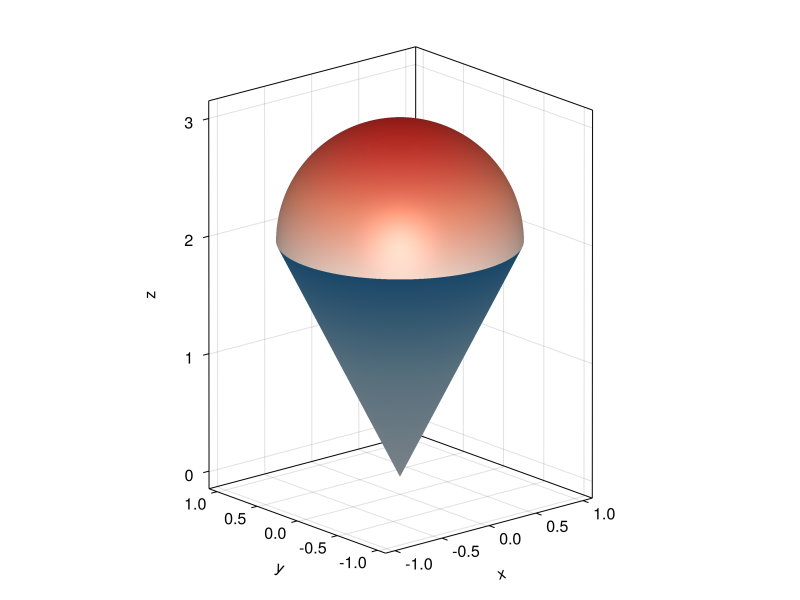
\includegraphics{img/examen-2023-12-22/helado.pdf}

\end{exercise}

\begin{tcolorbox}[enhanced jigsaw, coltitle=black, colbacktitle=quarto-callout-tip-color!10!white, bottomtitle=1mm, opacitybacktitle=0.6, breakable, bottomrule=.15mm, colframe=quarto-callout-tip-color-frame, toprule=.15mm, titlerule=0mm, arc=.35mm, colback=white, title=\textcolor{quarto-callout-tip-color}{\faLightbulb}\hspace{0.5em}{Solución}, leftrule=.75mm, rightrule=.15mm, opacityback=0, left=2mm, toptitle=1mm]

Despejando \(z\) de ambas ecuaciones, se tiene que la función que define
el cono es \(f(x,y) = 2\sqrt{x^2+y^2}\) y la que define la semiesfera
superior es \(g(x,y) = 2 + \sqrt{1-x^2-y^2}\), de manera que el volumen
del helado será el volumen comprendido entre las superficies de \(g\) y
\(f\).

Para determinar la región de integración, resolvemos la ecuación que
resulta de igualar las dos funciones.

\[
f(x,y) = g(x,y) \Leftrightarrow 2\sqrt{x^2+y^2} = 2 + \sqrt{1-(x^2+y^2)}
\]

Haciendo el cambio \(u^2=x^2+y^2\) se tiene

\[
\begin{gathered}
2 \sqrt{u^2} = 2 + \sqrt{1-u^2} 
\Leftrightarrow 2u-2 = \sqrt{1-u^2} \\
\Leftrightarrow 4(u-1)^2 = 1-u^2 \\
\Leftrightarrow 4u^2-8u+4 = 1-u^2 \\
\Leftrightarrow 5u^2-8u+3 = 0 \\
\Leftrightarrow u = 3/5 \mbox{ o } u = 1.
\end{gathered}
\]

Deshaciendo el cambio de variable, se tiene que la primera solución es
\(x^2+y^2=3/5\) y la segunda \(x^2+y^2=1\). Se observa que ambas
soluciones definen una región circular centrada en el origen con radios
\(\sqrt{3/5}\) y \(1\), respectivamente, ya que la esfera corta al cono
en dos planos distintos, pero tomaremos la última solución que es la que
se corresponde con la figura. Por tanto, la región de integración es
\(R=\{(x,y)\in \mathbb{R}^2: -1\leq x\leq 1, -\sqrt{1-x^2}\leq y\leq \sqrt{1-x^2}\}\).

Por las características de las funciones y de la región de integración,
resulta más sencillo hacer la integral en coordenadas polares, donde la
región de integración es
\(R=\{(r,\theta)\in \mathbb{R}^+\times \mathbb{R}: 0\leq \theta\leq 2\pi, 0\leq r\leq 1\}\).

\begin{align*}
\int_R g(x,y)-f(x,y) \,dA 
&= \int_0^{2\pi}\int_0^1 (g(r\cos(\theta), r\operatorname{sen}(\theta)) - f(r\cos(\theta), r\operatorname{sen}(\theta)))r\,dr\,d\theta \\
&= \int_0^{2\pi}\int_0^1 (2+\sqrt{1-(r\cos(\theta))^2-(r\operatorname{sen}(\theta))^2}-2\sqrt{(r\cos(\theta))^2+(r\operatorname{sen}(\theta))^2})r\,dr\,d\theta \\
&= \int_0^{2\pi}\int_0^1 (2+\sqrt{1-r^2}-2r)r\,dr\,d\theta \\
&= \int_0^{2\pi}\int_0^1 2r+r\sqrt{1-r^2}-2r^2\,dr\,d\theta \\
&= \int_0^{2\pi} \left[r^2-\frac{(1-r^2)^{3/2}}{3}-\frac{2r^3}{3}\right]_0^1\,d\theta \\
&= \int_0^{2\pi} 1-\frac{2}{3}+\frac{1}{3}\,d\theta \\
&= \int_0^{2\pi} \frac{2}{3}\,d\theta 
= \frac{2}{3}[\theta]_0^{2\pi}
= \frac{4\pi}{3}.
\end{align*}

Por otro lado, para averiguar la cantidad de barquillo que se necesita
para construir el cono del helado, hay que calcular el area de la
superficie del cono, que viene dada por la integral

\[
\int_R \sqrt{f'_x(x,y)^2+f'_y(x,y)^2+1}\,dA,
\]

donde \(R\) es la misma región de integración de antes.

Así que necesitamos calcular las derivadas parciales de \(f\).

\begin{align*}
f'_x(x,y)
&= \frac{2x}{\sqrt{x^2+y^2}} \\
f'_y(x,y)
&= \frac{2y}{\sqrt{x^2+y^2}}.
\end{align*}

Por tanto, hay que calcular la siguiente integral.

\begin{align*}
\int_R \sqrt{f'_x(x,y)^2+f'_y(x,y)^2+1}\,dA,
&= \int_{-1}^1\int_{-\sqrt{1-x^2}}^{\sqrt{1-x^2}} \sqrt{\left(\frac{2x}{\sqrt{x^2+y^2}}\right)^2 + \left(\frac{2y}{\sqrt{x^2+y^2}}\right)^2+1}\,dy\,dx \\
&= \int_{-1}^1\int_{-\sqrt{1-x^2}}^{\sqrt{1-x^2}} \sqrt{\frac{4x^2}{x^2+y^2} + \frac{4y^2}{x^2+y^2}+1}\,dy\,dx \\
&= \int_{-1}^1\int_{-\sqrt{1-x^2}}^{\sqrt{1-x^2}} \sqrt{5}\,dy\,dx \\
&= \int_0^{2\pi}\int_0^1 \sqrt{5}r\,dr\,d\theta \tag{1}\\
&= \int_0^{2\pi}\sqrt{5}\left[\frac{r^2}{2}\right]_0^1\,d\theta \\
&= \int_0^{2\pi}\frac{\sqrt{5}}{2}\,d\theta
= \frac{\sqrt{5}}{2} [\theta]_0^{2\pi}
= \sqrt{5}\pi.
\end{align*} (1) Cambio a coordenadas polares.

\end{tcolorbox}



\end{document}
